\chapter{动态延迟感知的2.5维堆叠\\片上网络负载均衡策略}
\label{chap:DLL}
本章针对2.5维堆叠片上网络出现的负载不均衡问题,提出了一种动态延迟感知的2.5维堆叠片上网络结构负载均衡策略。
\ref{sec:dllbackground}节和\ref{sec:dllrelated}节介绍了本章的研究背景和相关工作。
\ref{sec:dlldesign}节给出了本章的负载均衡策略及拥塞信息传输环网。
\ref{sec:dllexperiment}节介绍了本章的实验方法和实验结果。
\ref{sec:dlldiscussion}节和\ref{sec:dllconclusion}节分别讨论了一些工作细节并总结全章工作。

\section{研究背景}
\label{sec:dllbackground}

近年来,基于硅中介层的堆叠,即2.5维堆叠~\upcite{deng2001interconnect}越来越受到业界的重视~\upcite{loh2015interconnect}。
如图~\ref{fig:interposer}所示,2.5维堆叠技术将多个晶粒一起堆叠在硅中介载体上。
由于三维堆叠是一种革命性的技术,需要全新的设计、测试方法以及工具,2.5维堆叠则是一种相对渐进的技术~\upcite{bolsens20112}。
2.5维堆叠技术可以避免很多三维堆叠技术面临的挑战,并且能够被当前的设计工具链支持。
此外,当前的堆叠存储系统为每个堆叠存储单元提供了固定的带宽和容量标准。
相比于三维堆叠技术,硅中介层有足够的面积来集成更多的堆叠存储单元,能够达到更高的总存储带宽和更大的存储容量~\upcite{loh2015interconnect}。
因此,近几年的商业化2.5维堆叠产品已经开始变得越来越流行~\upcite{AMD2015USER,saban2011xilinx,pascal}。

\begin{figure}[htbp] % use float package if you want it here
  \centering
  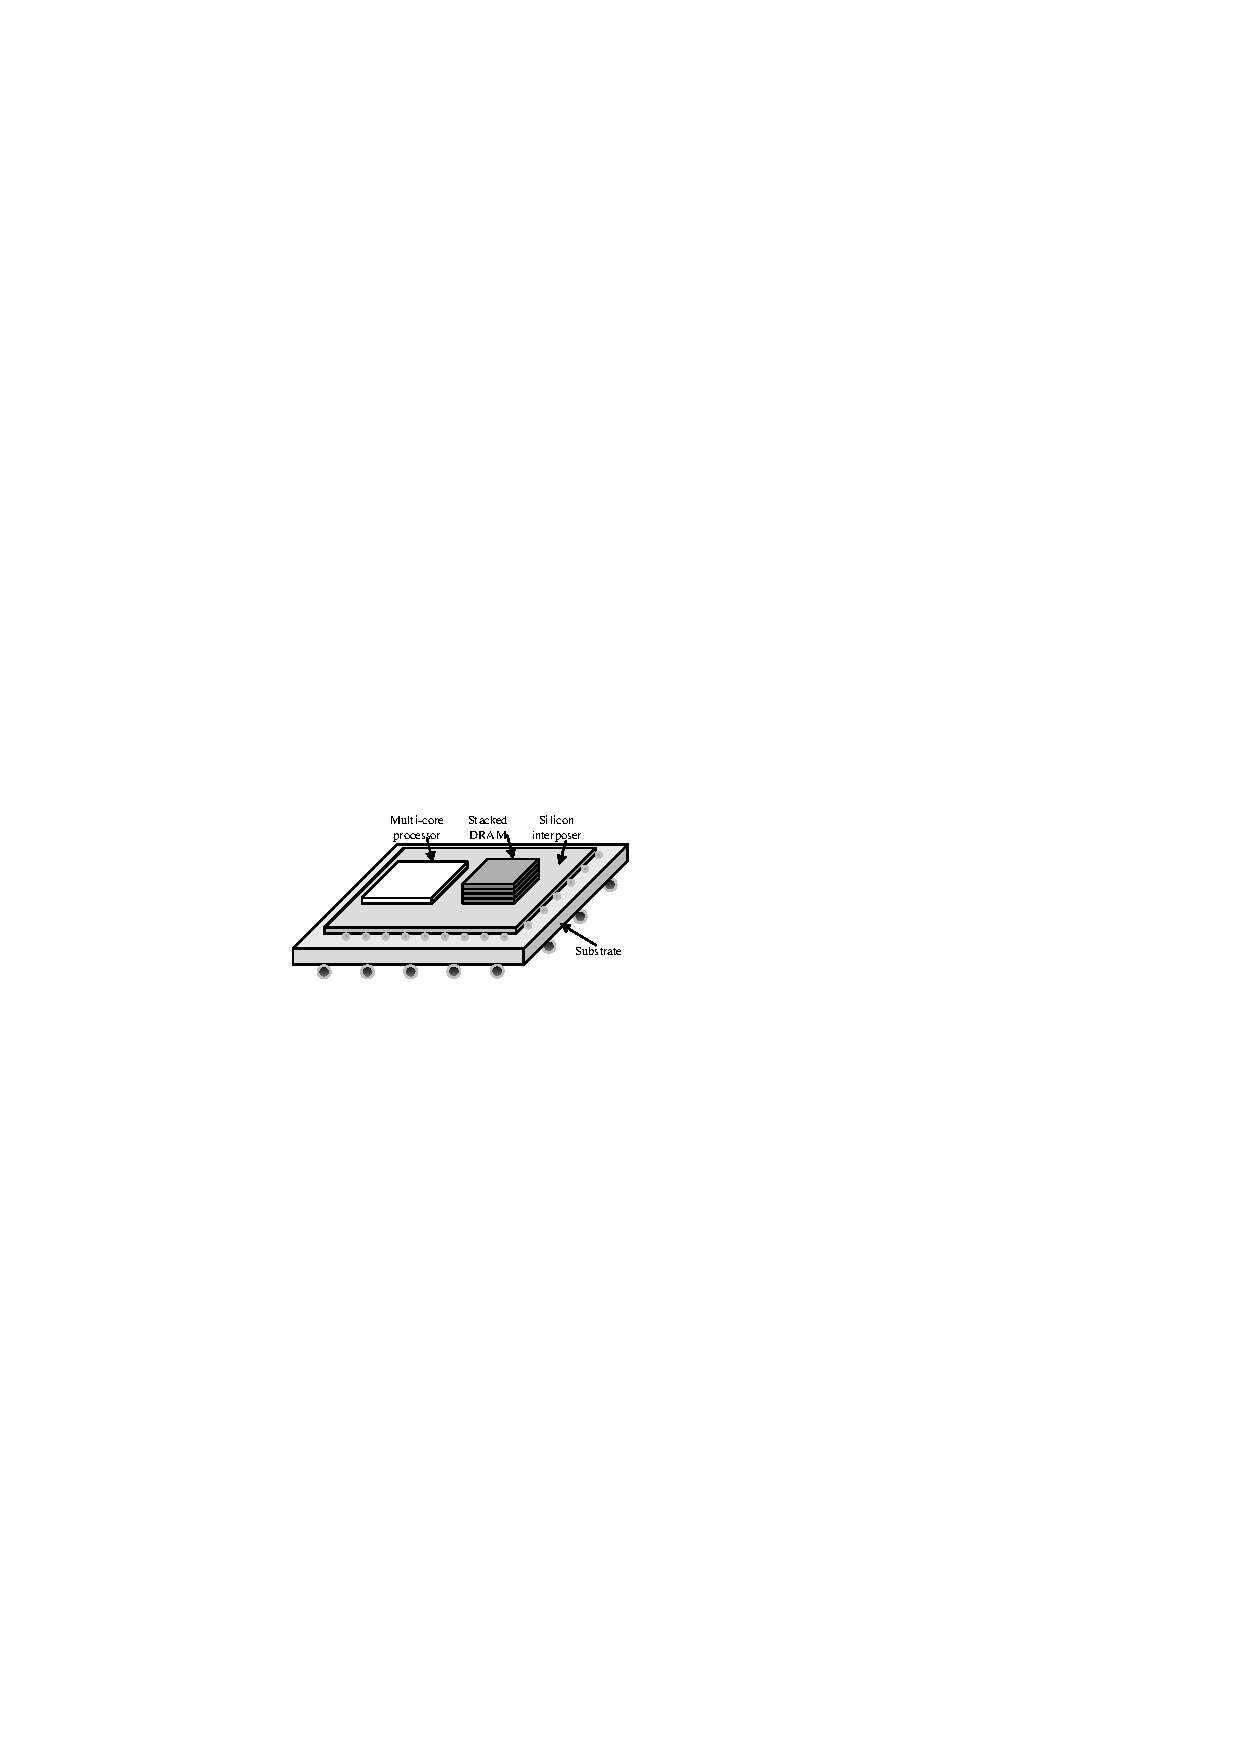
\includegraphics[width=.8\textwidth]{/Figs_DLL/interposer}
  \caption{2.5维堆叠技术}
  \label{fig:interposer}
\end{figure}

为了更加高效的满足2.5维堆叠系统的通信要求,之前的工作~\upcite{jerger2014noc,loh2015interconnect,kannan2015enabling}显示硅中介层上有足够的连线资源,这些连线资源可以进一步被开发以实现另一层片上网络。
当2.5维堆叠硅中阶层系统上存在两层片上网络时,比较可取的方式是将核间协议的通信和访存通信划分开~\upcite{jerger2014noc}。
因为这两种通信特性非常不一样,将这两种通信划分到不同的网络层有许多优势。

但是,本章用PARSEC测试集在基准2.5维堆叠结构上测试,发现访存通信平均仅占全部通信的14.8\%。
这些应用程序的核间通信量远大于访存通信量,出现极大不均衡性。
核间通信的网络层出现拥塞,而另一层则未被充分利用。
这将导致较差的性能。
因此,需要一种2.5维堆叠片上网络的负载均衡策略来平衡两个网络层的负载,并将资源利用率最大化。

\texttt{缓存感知}和\texttt{延迟感知}的方法是比较通用的均衡多层网络负载的方法。
传统的\texttt{缓存感知}的方法通过邻居节点的缓存占用率来收集和判断拥塞信息~\upcite{das2013catnap,gratz2008regional}。
但是,这种局部的拥塞信息无法完全反映全局的拥塞状态,因此并不适合用于指导2.5维片上网络的网络选择。
我们知道,基于目的节点检测的\texttt{延迟感知}方法是目前2.5维片上网络唯一的负载均衡策略。
它在目的节点收集每个报文的传输延迟来检测该节点的拥塞信息,并为该节点发出的报文选择网络层~\upcite{jerger2014noc}。
但是,这种策略采用的是不精确的信息,因为对于每个节点报文接收的路径和报文发送的路径是不一样的。
该方法采用了报文接收的路径的拥塞情况来代表报文发送路径的拥塞情况。
如图~\ref{fig:dest_src}所示,节点10收集的接收报文延迟,即绿色路径作为拥塞信息。
但是,该节点发送的报文是沿红色路径传输的。

\begin{figure}[htbp] % use float package if you want it here
  \centering
  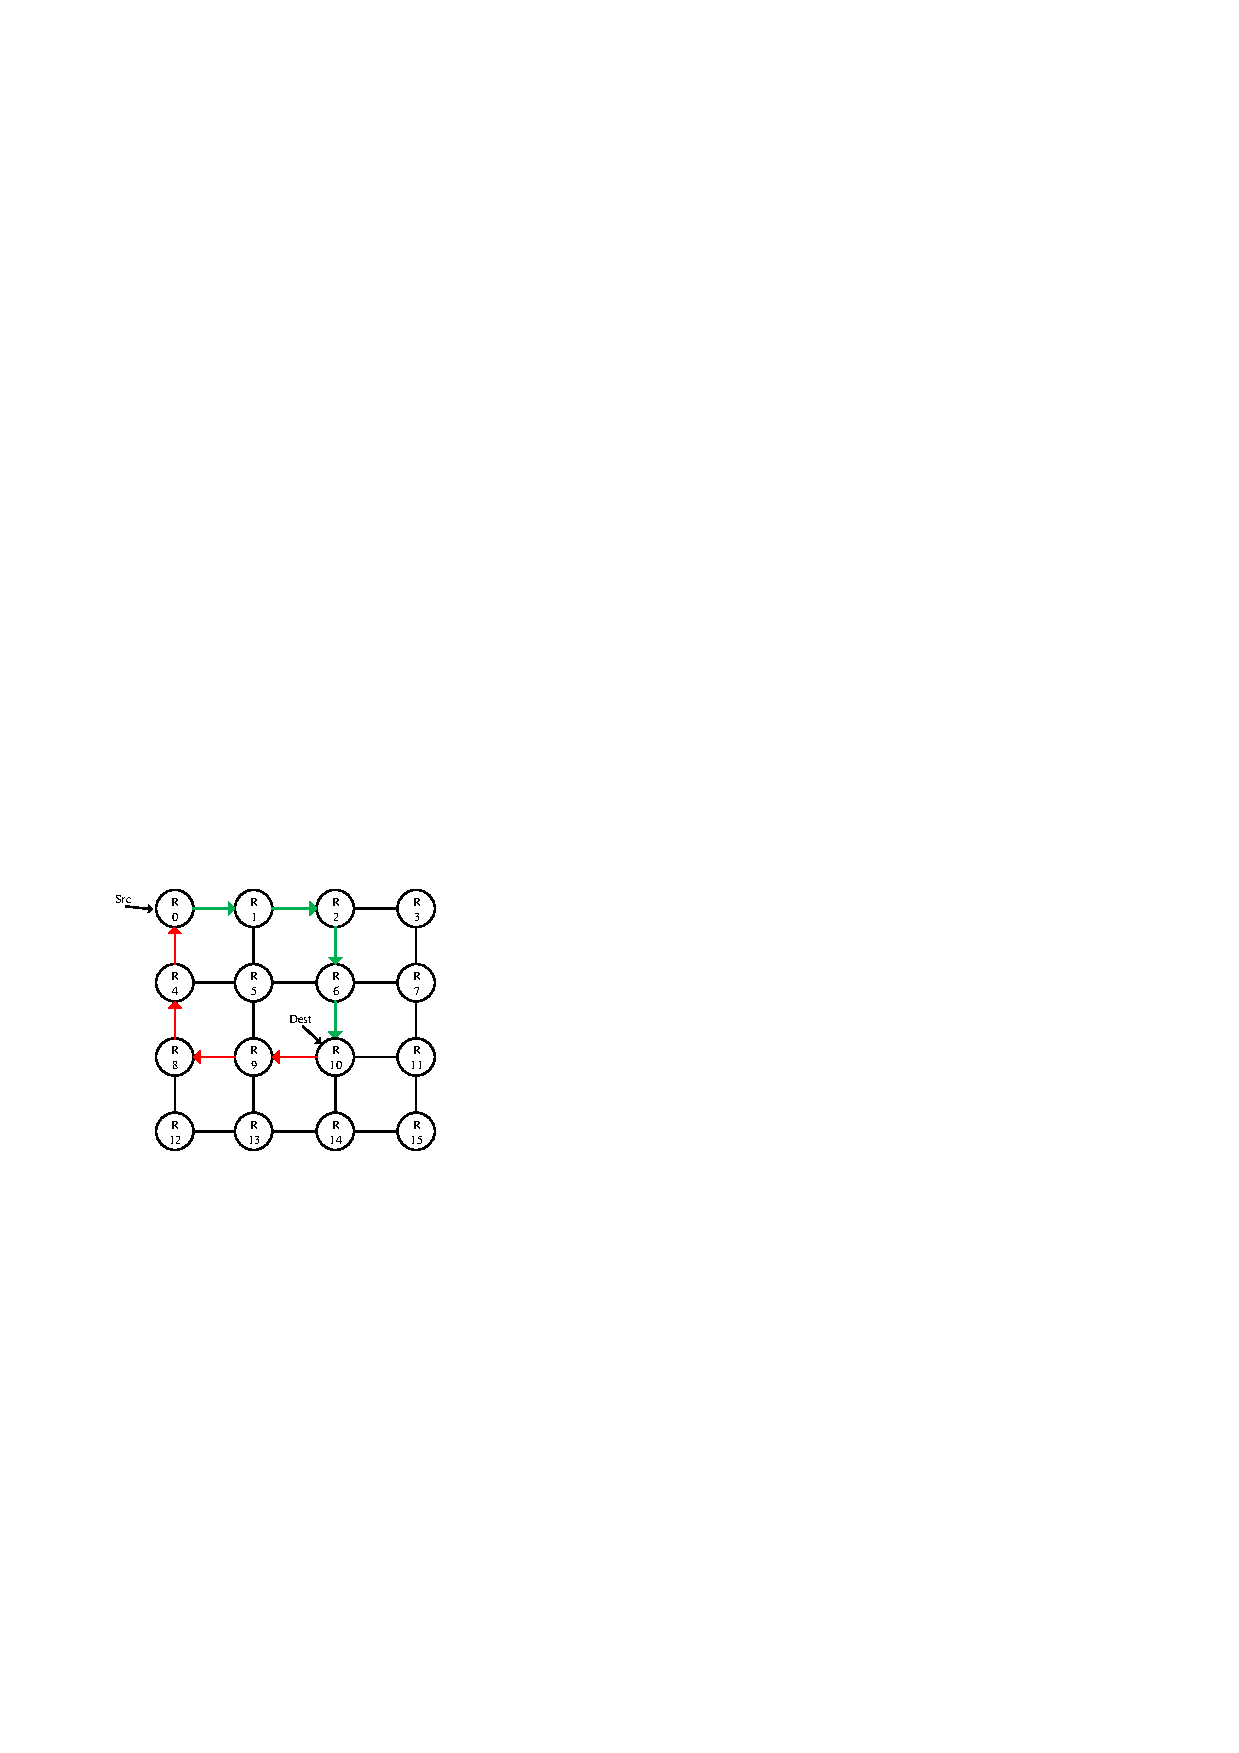
\includegraphics[width=.7\textwidth]{/Figs_DLL/dest_src}
  \caption{目的节点检测的负载均衡策略(采用XY路由算法,绿线为拥塞信息收集的路径,而红线则是节点10发送报文到节点0所走的路径。
  在这种情况下,从绿色路径收集的拥塞信息会被当做红色路径的拥塞信息提供给源节点10作为拥塞控制依据。)}
  \label{fig:dest_src}
\end{figure}

需要研究合适的拥塞检测机制来获取准确的网络状态,并做出高效的网络选择。
这是实现2.5维片上网络负载均衡的基础。

本章提出了2.5维片上网络结构的动态延迟感知负载均衡策略(DLL)。
DLL策略首先收集每个目的节点的拥塞信息。
然后,通过DLL的延迟传输环网,将拥塞信息传输回源节点。
最后,每个源节点通过收到的拥塞信息选择网络层来传输报文,DLL策略包括以下几个主要贡献:
\renewcommand*\theenumi{(\alph{enumi})}
\begin{enumerate}
\setlength\itemsep{1pt}
\item 本章评估并分析了PARSEC测试集的通信流量,发现2.5维片上网络的通信流量在两个网络层极不公平,
急需一种高效负载均衡策略。

\item 本章分析了当前负载均衡策略的缺点。
缓存感知的方法无法获取全局网络的拥塞状态。
当前的延迟感知方法不能准确的检测全局拥塞状态。

\item 本章提出了一种2.5维片上网络的动态延迟感知的负载均衡策略。
这个策略在目的节点收集拥塞信息,并将这些拥塞信息传输回源节点用于网络选择。
本章还设计了一个多链路无阻塞的环网用于传 输这些拥塞信息。

\item 与没有负载均衡的基准2.5维片上网络结构,当前的延迟感知方法以及缓存感知方法相比,DLL策略两个平均提升45\%、14.9\%和6.5\%的吞吐量,而开销则非常低。
\end{enumerate}

\section{相关工作}
\label{sec:dllrelated}

由于2.5维堆叠技术展现在带宽、延迟和开销上的突出优势,近些年来一系列2.5维堆叠的工业界产品被推出。
第一个发布的2.5维堆叠商业产品是Xilinx Virtex-7 2000T FPGA~\upcite{saban2011xilinx},该平台是由四块相对较小的FPGA堆叠在硅中介层上形成的。
High Bandwidth Memory (HBM)~\upcite{hbm2,lee-taco2016}和Hybrid Memory Cube(HMC)~\upcite{hmc1,hmc2}是两个比较先进的堆叠存储技术,它们已经被广泛应用到2.5维堆叠的处理器中。
当前,他们能够提供每个堆叠单元128GB/s的带宽。
AMD Radeon R9 Fury Xnew GPU 在其2.5维堆叠结构中采用了HBM作为存储单元以提供超大的带宽和容量\upcite{AMD2015USER}。
NVIDIA PASCAL GPU体系结构则采用了第二代HBM\upcite{pascal,nvi2015pascal}。
2.5维堆叠技术和第二代HMC也将被应用到下一代的Intel Xeon Phi协处理器中\upcite{Micro2015intel}。

Enright Jerger等人的工作是第一个提出开发基于硅中介层的片上网络互连设计空间的~\upcite{jerger2014noc}。
他们比较了几种拓扑逻辑结构,提出了一种负载均衡策略。
但是,他们的策略收集目的节点的拥塞信息(延迟),并将目的节点的拥塞信息用于指导目的节点的报文发送及网络层的选择。
由于报文的发送路径和接收路径并不相同,这个策略采用的实际上是不精确的网络状态信息进行网络层选择。
这个策略在本章中将被称为DestDetect。

在传统的二维片上网络中,关于拥塞控制的工作非常多。
Li等人提出DyXY路由机制基于本地网络拥塞状态~\upcite{li2006dyxy}。
相对于静态路由方法,该方法可以达到更高的性能。
RCA~\upcite{gratz2008regional}是第一个采用了本地和非本地信息来实现负载均衡的工作。
但它在拥塞计算上引入了干扰和冲突。
DBAR~\upcite{ma2011dbar}通过在收集拥塞信息时保持动态独立解决这个问题。
所有这些方法都应用了缓存利用率的统计作为拥塞信息。
而缓存利用率作为拥塞信息更适合路由路径的选择而不是网络层的选择。

在三维片上网络结构或者是多片上网络结构的负载均衡问题上,Ranmanujam等人提出了一种高效的层多路复用(LM)三维结构~\upcite{ramanujam2009layer}。
他们通过在垂直方向上的多路复用和多路分解结构,替代了传统三维片上网络结构上的一层一跳步的通信方式。
在负载均衡逻辑中,每一对输入输出端口采用了一套切片计数器进行拥塞判断和网络层的选择。
这种拥塞信息反映了网络层的通信流量,但网络层中的热点区域无法被检测到。
Catnap~\upcite{das2013catnap}是一种高能效比的多网络结构,该结构的子网络可以通过门控时钟(Power gating)技术关掉,不需要考虑网络连接性。
他们实现了一种基于拥塞状态观察的子网选择策略。
通过计算每个路由器输入缓存的缓存占用率来检测拥塞。
然而,这种方法不能反映全局拥塞状态,在本章中该拥塞检测和网络选择策略称为LocalBuf策略,将与本章提出的DLL策略进行比较。


\section{设计}
\label{sec:dlldesign}

本节首先介绍了2.5维堆叠片上网络的目标系统。
之后本节分析了片上网络的通信和拥塞特性来解释DLL的设计动机。
最后从两个方面介绍DLL策略,一方面是拥塞控制和网络选择策略;另一方面是延迟传输环网。

\subsection{目标系统}
\label{sec:dlltarget}

DLL策略可以广泛地应用到基于硅中介层的系统和多网络层系统的选择,因此本章展示了一个例子以更方便具体的呈现DLL策略。
本章的2.5维堆叠硅中介层系统集成了64核的CPU,其周围集成了4个堆叠DRAM存储器。
在这个系统中包含两个网络层,上面一层是CPU层,而下面一层是硅中介层。
这两个网络层通过TSV和$\mu$bump互连。
如图~\ref{fig:target_system}所示,本章的2.5维堆叠片上网络结构,在CPU层的拓扑逻辑是MESH。
由于$\mu$bump会引入较大的开销~\upcite{liu2011vertical},在硅中介层,本章采用了集中式MESH以减小路由器数量。
在硅中介层中共有16个节点,每个节点连接4个CPU节点。
在硅中介层网络的两侧总共有8个访存控制器。
每个访存控制器包含两个DRAM通道,连接到相邻的硅中介层节点。
图~\ref{fig:target_system}也展示了两种类型的硅中介层实现,包括主动式和被动式。
相比于主动式的硅中介层,被动式的硅中介层不包含有源器件(逻辑、门)。
所有的硅中介层路由器都实现在CPU层。
短期来看,被动式的硅中介层仍然是一种比较现实的方案,而主动式的硅中介层则更像是一种三维堆叠的方式。

\begin{figure}[htb]
\centering
\subfloat[顶视图]{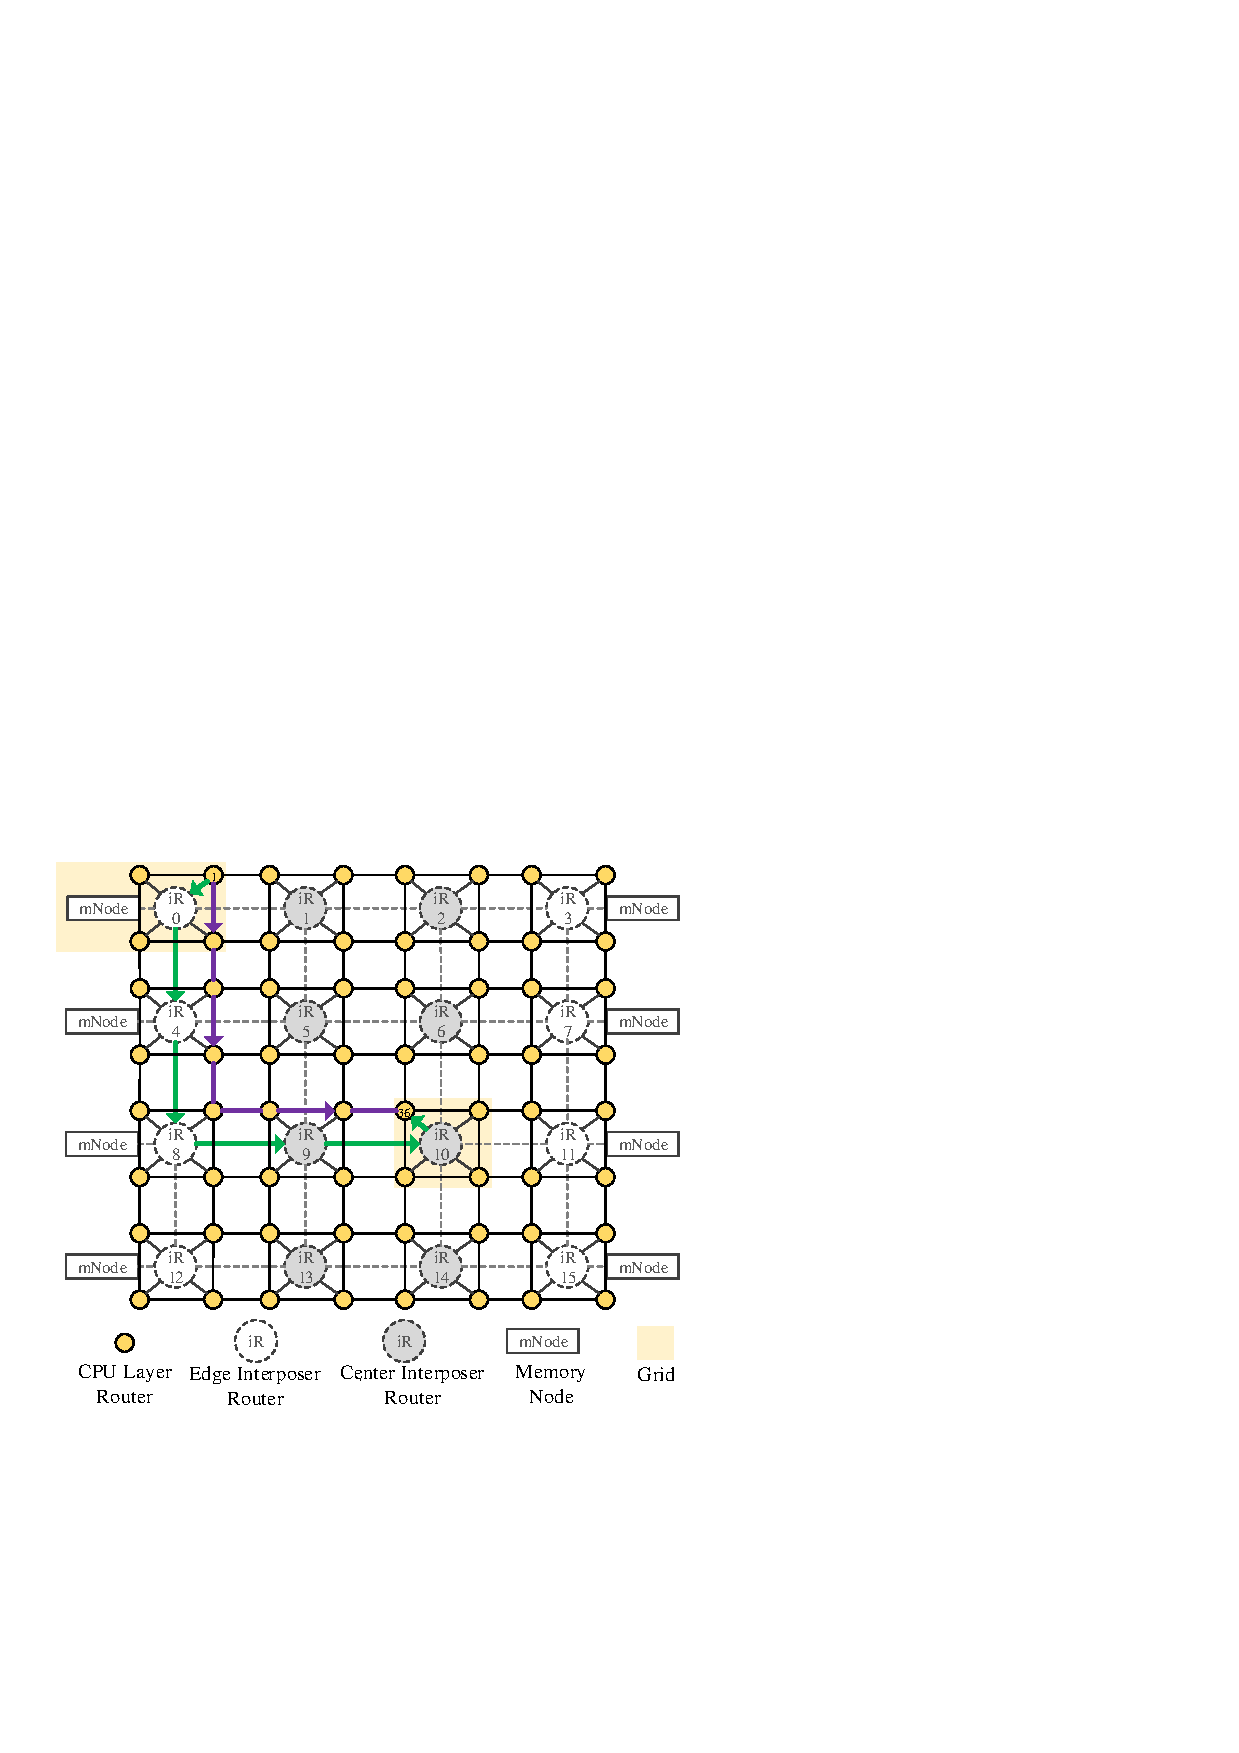
\includegraphics[width=.7\textwidth]{/Figs_DLL/target_system}} \qquad
\subfloat[侧视图(有源硅中介层)]{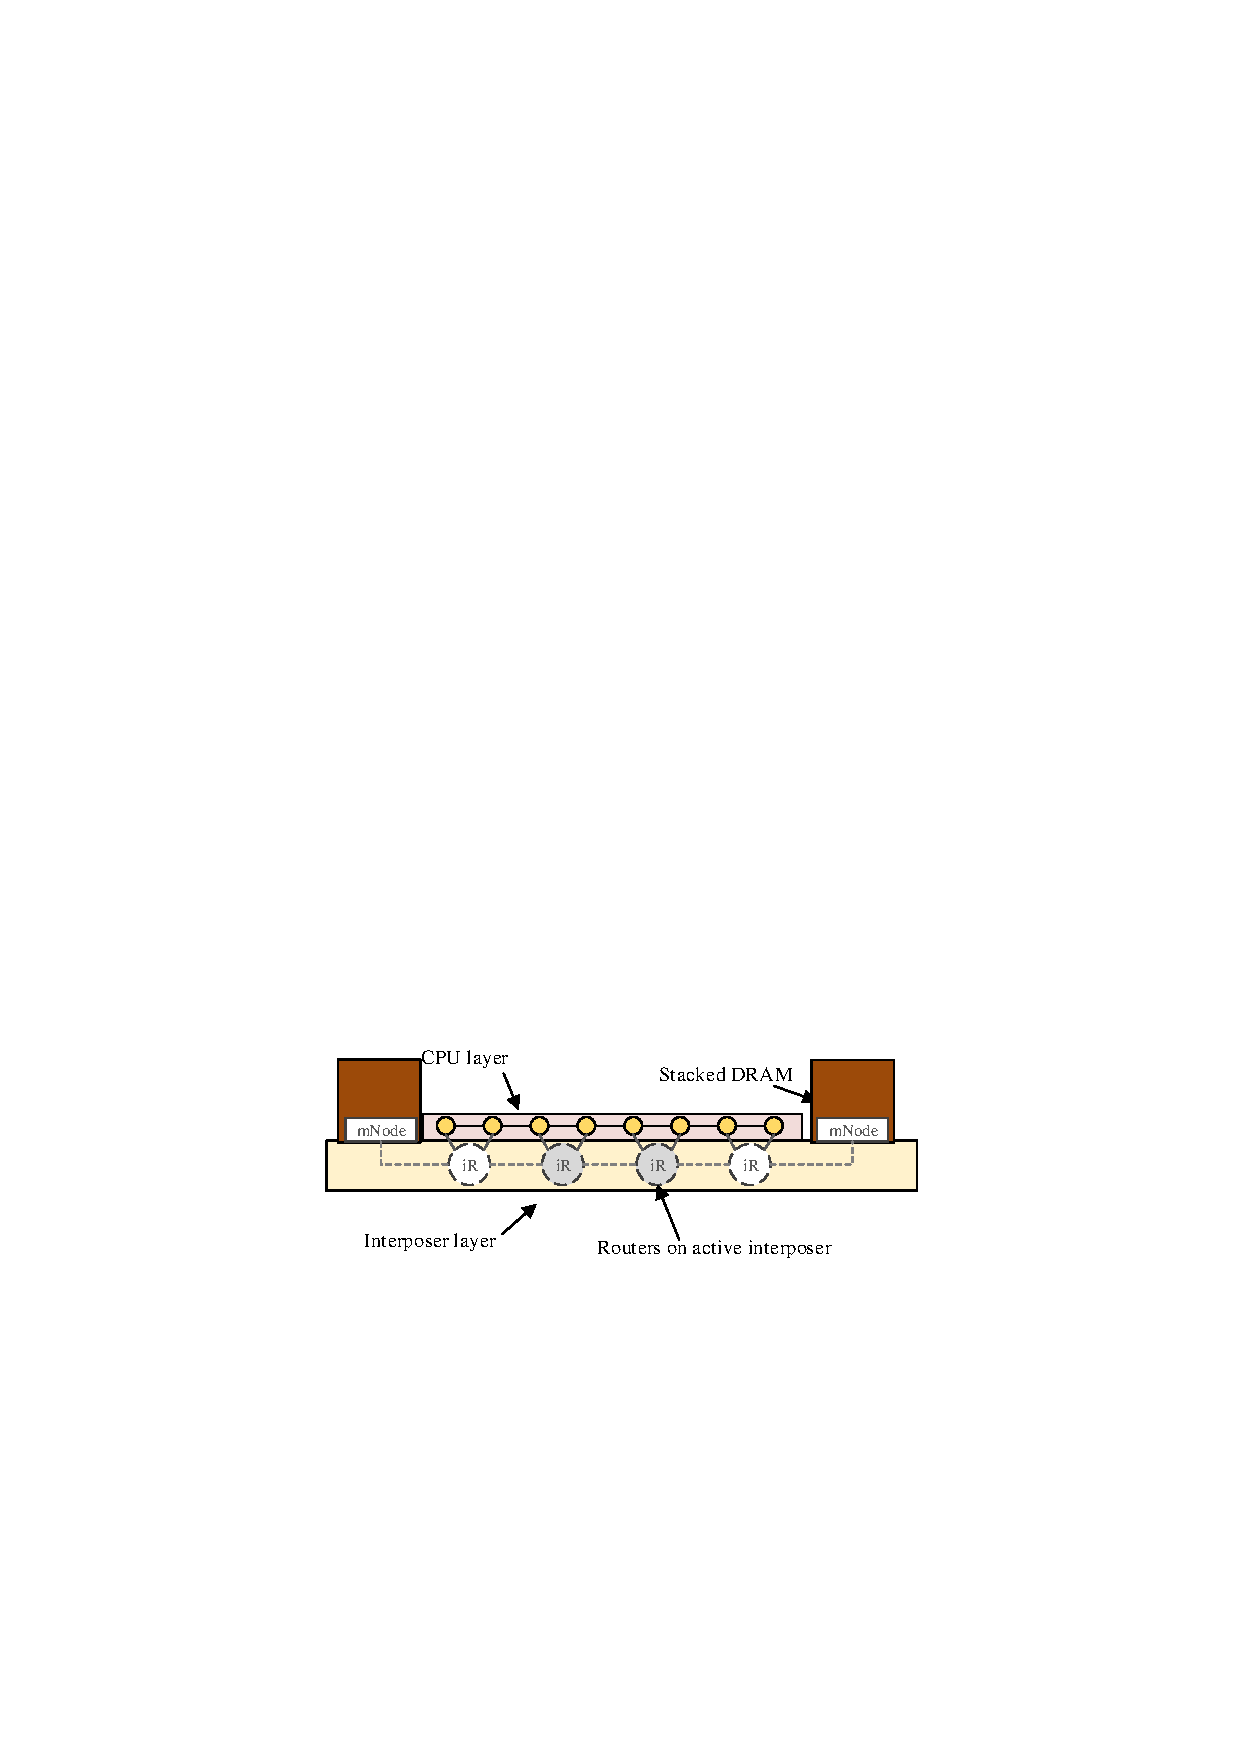
\includegraphics[width=.7\textwidth]{/Figs_DLL/target_system_active}} \qquad
\subfloat[侧视图(无源硅中介层)]{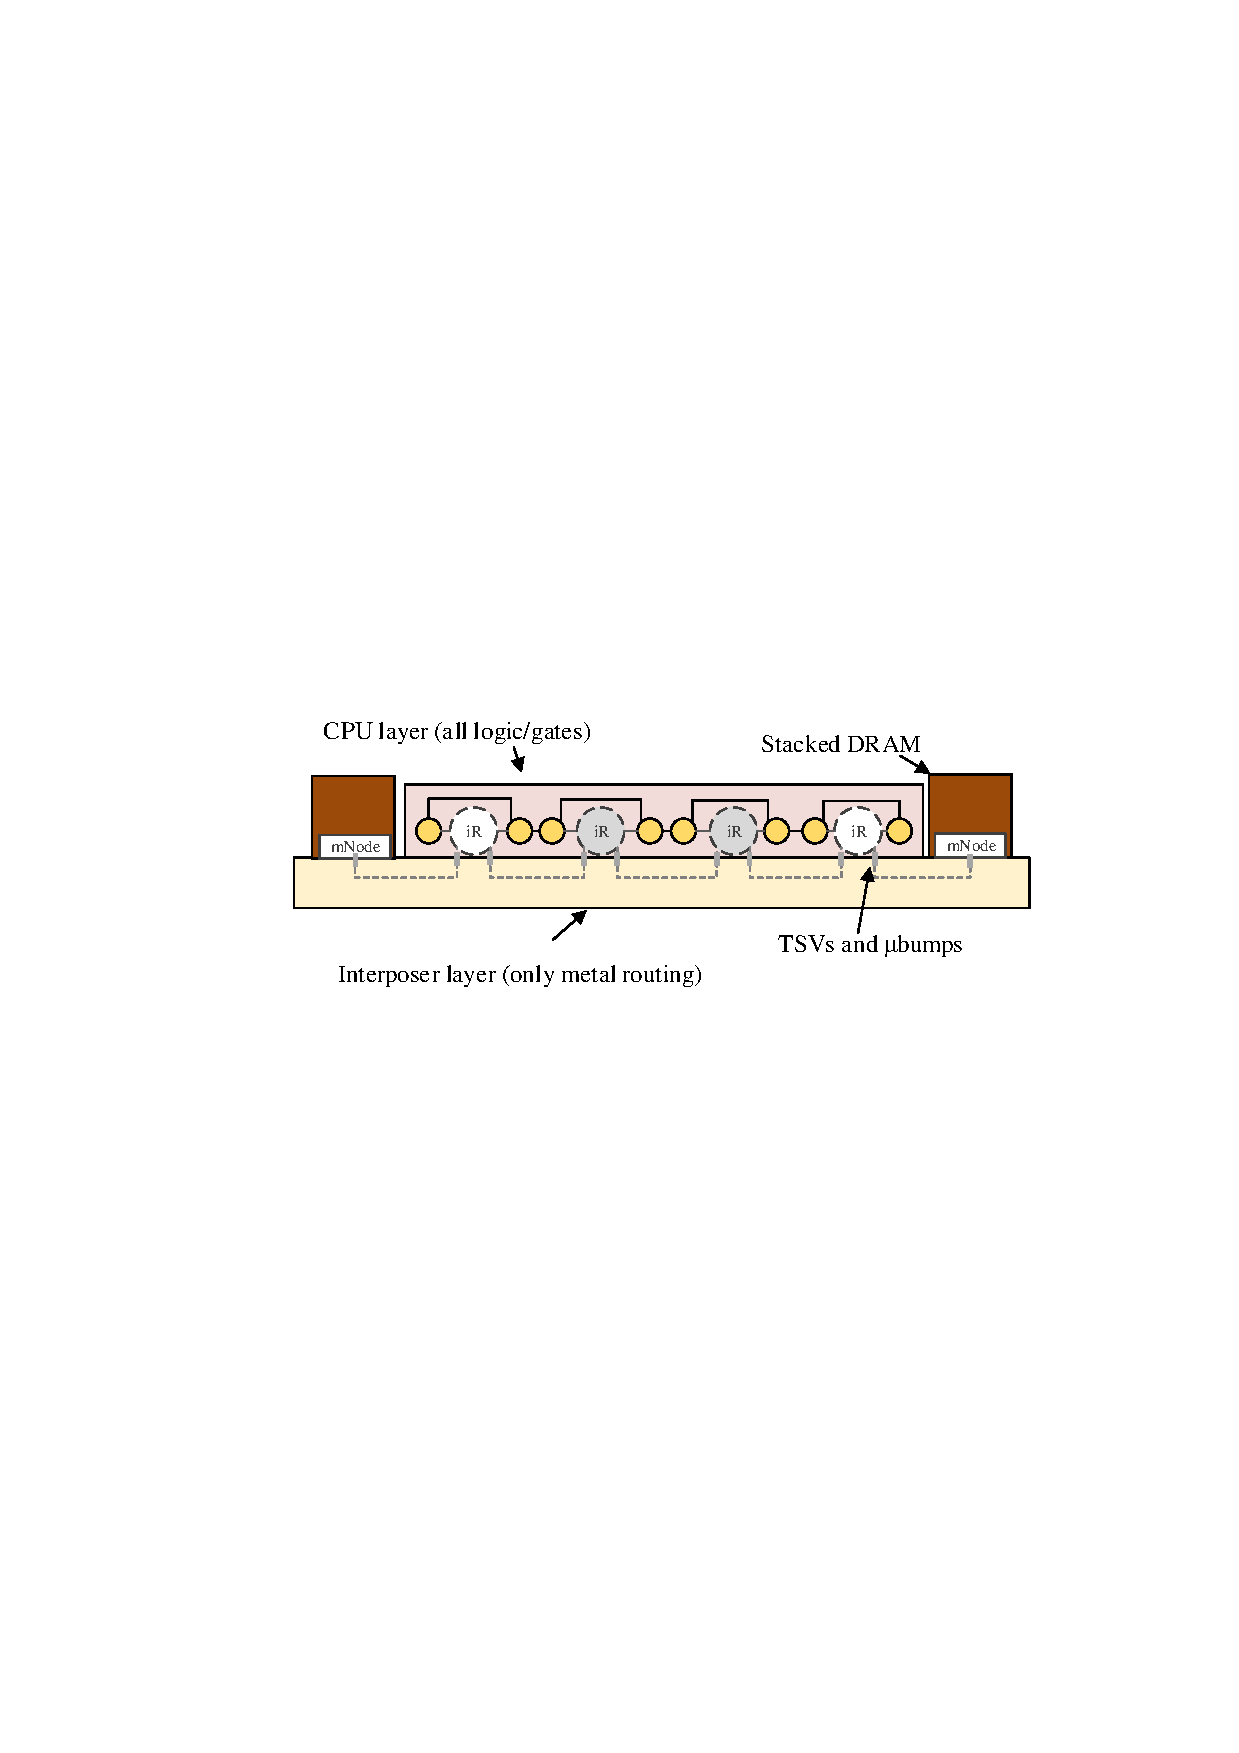
\includegraphics[width=.7\textwidth]{/Figs_DLL/target_system_passive}}  
\caption{2.5维片上网络结构的目标系统}
\label{fig:target_system}
\end{figure}

在目标系统中,包含两种类型的通信,核与核之间的通信以及核与存储之间的通信。
之前的研究表明,将这两种通信划分到不同的两层网络上会带来许多优势~\upcite{jerger2014noc}。
核间协议通信在CPU层传输,而核与存储之间的访存通信则可以在硅中介层上进行。
但是,这种片上网络通信的划分并不是非常严格的。
这依赖于应用程序的需要以及真实片上网络结构的应用。
在下一节,将介绍DLL的负载均衡策略。
该策略基于拥塞状态来划分片上网络的通信流量的传输层次。


\subsection{设计原则}

本章分析片上网络的通信和拥塞特性。
这些特性对于设计一个负载均衡策略尤为重要。
根据通信和拥塞特性,本章也给出了2.5维堆叠片上网络结构负载均衡策略的两个设计原则。

\textbf{通信特性}:许多应用程序(包含PARSEC和SPLASH-2测试集),都呈现出相对不均衡的特性。
在空间特性上,多数的通信流量都是在几对节点之间进行的,大多通信报文都是在几对节点之间传输,与合成流量模型的Permutation流量模式类似。
因此负载较重的流量的通信路径可以通过报文延迟清晰地反映出来。

\textbf{设计原则1}:以每个路由器的缓存占用率作为拥塞度量,可以反映路由器的拥塞状态。
每个节点只能检测到本地拥塞的状态。
当该网络层部分区域拥塞,部分区域不拥塞时,无法针对特定报文的路径对网络拥塞进行判断。
相反,最近的几个报文的平均通信延迟可以反映出针对特定报文的网络相应路径的拥塞情况。
因此,网络层中的全局拥塞状态可以通过延迟感知的方式被更准确地检测。
本文采用延迟感知的方法进行拥塞检测而不是缓存感知的方法。

\textbf{拥塞特性}:片上网络的通信呈现出类似Permutation通信模式的特点。
较重负载的通信路径会很容易变得拥塞,而负载较轻的通信路径则会未被充分利用。
对于负载较重的通信路径经过的节点,整个网络层是拥塞的;
而对于负载较轻的通信路径经过的节点,整个网络层是未被充分利用的。
因此,从不同的节点观察整个网络的拥塞情况,同一个网络层可能是拥塞的也可能是不拥塞的。

\textbf{设计原则2}:由于不同的节点可能观察到同一个网络层不同的拥塞状态,需要采用源节点观察到的拥塞信息用于同一节点的网络层选择。
如果该信息用在了目的节点的报文发送上,不准确的拥塞路径将被反映出来。
如果从全局的角度来看,这种整个网络层不均匀的拥塞状态无法被直接反映出来。
网络层中较轻负载的路径可能会被认为是拥塞路径,反之亦然。
因此,网络选择最好是在源节点做决定,而不是目的节点或从全局视角。

本章利用了延迟感知的方法来检测全局网络层的拥塞,并为2.5维片上网络层中选择合适的网络层进行传输。

\subsection{拥塞检测和网络选择}

上述设计原则的指导下,本章开发了DLL策略。
该策略采用最近几个报文的延迟作为网络拥塞的衡量指标。
在源节点比较两层网络的平均报文延迟用于网络选择。
如图~\ref{fig:target_system}(a)所示,如果节点1发送报文给节点36,节点1首先要比较从节点1发送到两层网络的报文的平均延迟。
如果上层网络的平均延迟大于下层网络的延迟且超出一定阈值,则报文会被路由通过绿色路径达到负载均衡,而不是紫色路径。

从技术上看,DLL策略需要实现3个关键问题:

1)如何在路由器记录报文的延迟?

2)如何产生并传输拥塞信息?

3)如何根据拥塞信息作出网络层的选择?

DLL策略主要包含四个设计的细节。

首先,由于因为报文传输距离较远时,通信延迟肯定长于较短距离的传输,因此采用报文的总传输延迟并不公平,并且可能会误导我们做出错误的网络选择。
本文比较不同报文的单跳平均延迟来选择网络层。
延迟信息会被记录在每个报文的头切片上。

第二,如果传输所有报文的延迟信息回源节点,其开销是无法容忍的。
因此,DLL策略采用了粗粒度的方法。
网络会被划分为多个格子,每个格子包含多个节点,同一个格子内的节点的拥塞信息将被合并以降低开销。
如图~\ref{fig:target_system}(a)所示,如果节点1发送报文到节点36,本章的粗粒度策略认为该报文是从格子0发送到格子10。
我们将连接着同一个硅中介层节点的4个CPU节点视为一个格子,如图~\ref{fig:target_system}(a)显示的黄色块描述的。
边界的存储节点也被包括在格子内。
格子的序号和硅中介层节点的序号是一样的。

第三,因为所有的存储控制器都分布在硅中介层水平方向的两侧,2.5维堆叠下层网络的边界可能成为瓶颈。
本章采用YX-Z路由代替XY-Z路由来降低边界节点的通信压力。
通过这个方法,经过边界的路由到达目的存储控制器的报文数量将减少。

第四,DLL策略可以消除协议层和网络层的死锁。
协议层死锁可以通过虚通道来避免,而网络层死锁则通过维序路由来消除。
即使报文会从一个网络层传输到另一个网络层,本章依然能够保证无死锁,这是因为Z跳一定是第一跳步或者最后一跳步,不可能形成环。

拥塞检测和网络选择总共有5个步骤,如图~\ref{fig:procedure}所示。

\begin{figure}[htbp] % use float package if you want it here
  \centering
  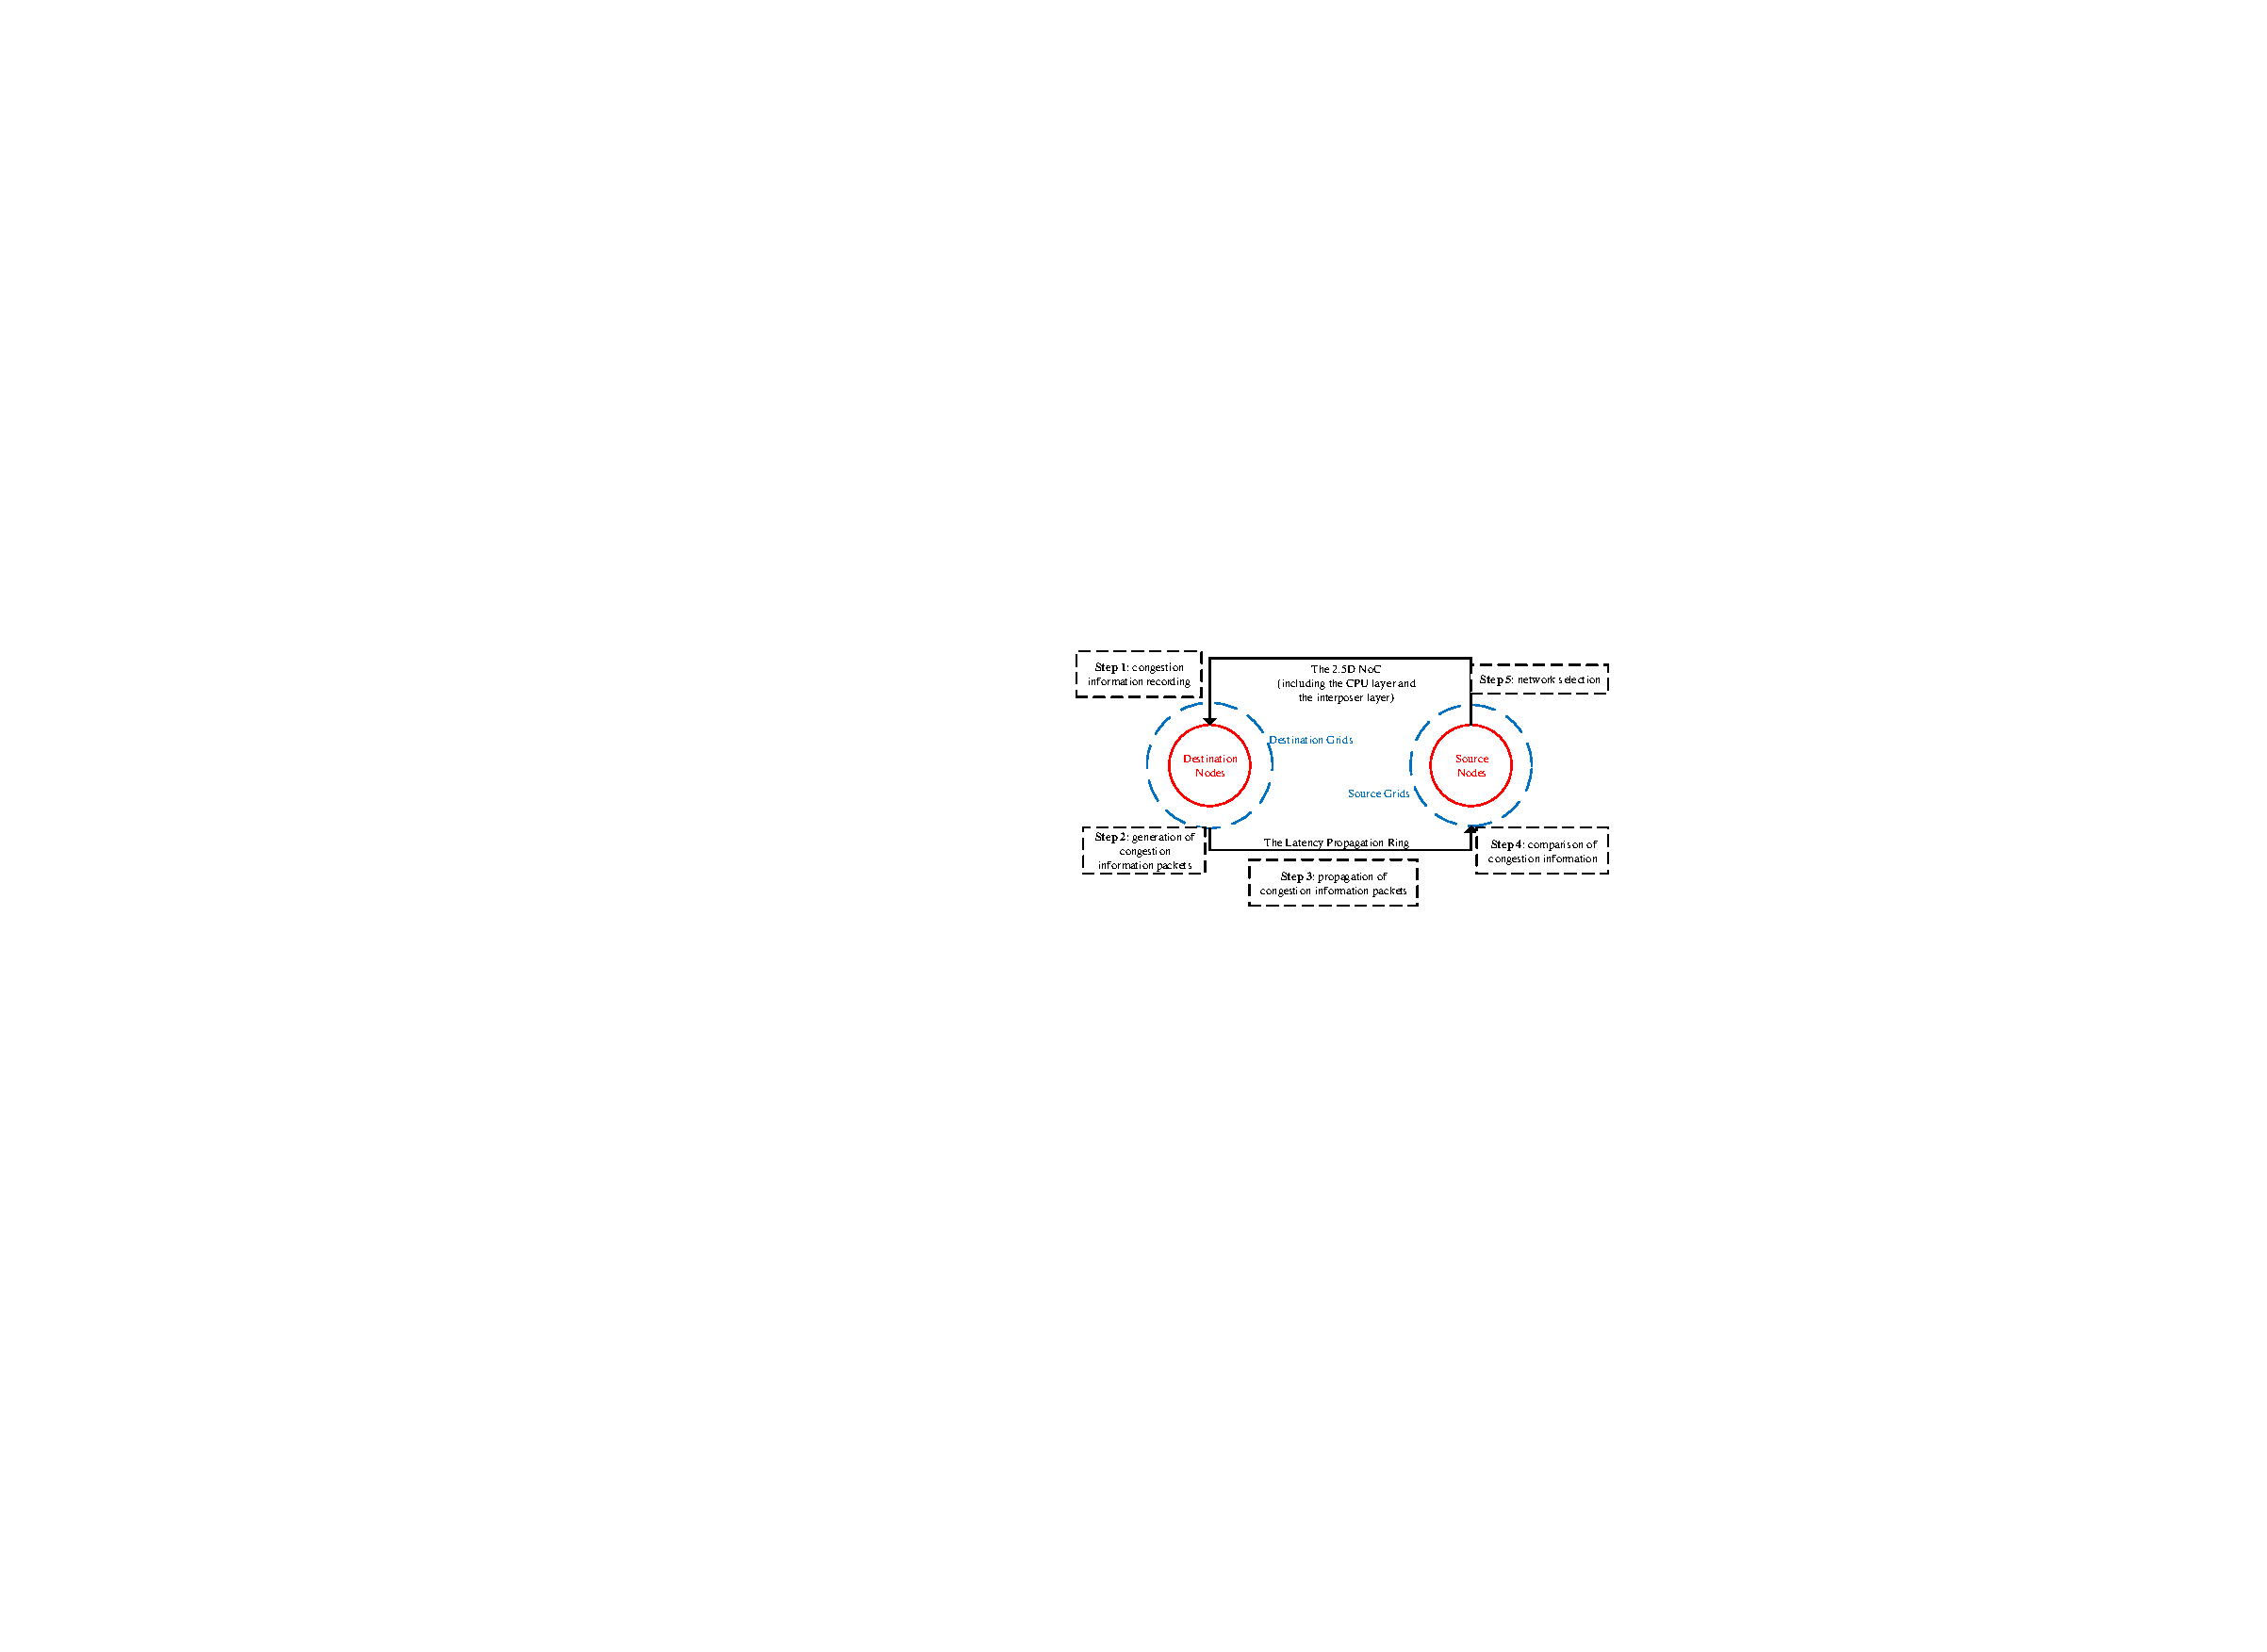
\includegraphics[width=\textwidth]{/Figs_DLL/procedure}
  \caption{DLL策略的工作流程}
  \label{fig:procedure}
\end{figure}

第一步在目的节点记录报文延迟。本章为每个报文增加了一个域记录延迟。
延迟可以通过每个路由器的时钟来收集。
一旦头切片准备完毕可以发送,该域按如下公式进行更新:

$$ L =
\dfrac{L_{last}\times hop + t _{out}-t _{in}}{hop+1} , \eqno(1)
 $$

其中\emph{L}$_{last}$是上一跳之前的平均跳步延迟。
\emph{L}是当前跳步之前的平均跳步延迟,\emph{hop}是当前跳步数,\emph{t}$_{out}$是本地路由器发送出该报文的时间,\emph{t}$_{in}$是该路由器收到该投切片时的时间。
当收到一个报文时,目的节点首先计数该报文的每一个跳步的平均延迟。
如果平均延迟大于15\emph{(2‘b1111)},则将被记录为15\emph{(2‘b1111)}。
我们相信每跳步15个时钟周期已经足以表明其拥塞状态。
由于每个跳步的延迟只需要4位来表示,因此计算将非常简单和快速。

第二步是在目的格子产生包含拥塞信息的报文。
三种类型的数据将被打包存入仅需9位的拥塞信息报文,如图~\ref{fig:congest_packet}所示,包括了源格子,平均跳步延迟以及传输层。
传输层被编码为0代表上层,编码1代表下层。
目的节点发送拥塞信息报文到属于同一格子的硅中介层节点。
如果硅中介层的节点的缓存已满,新产生的拥塞信息将被直接丢弃。
DLL策略采用的粗粒度方法,并不会严重影响拥塞信息收集的准确度。

\begin{figure}[htbp] % use float package if you want it here
  \centering
  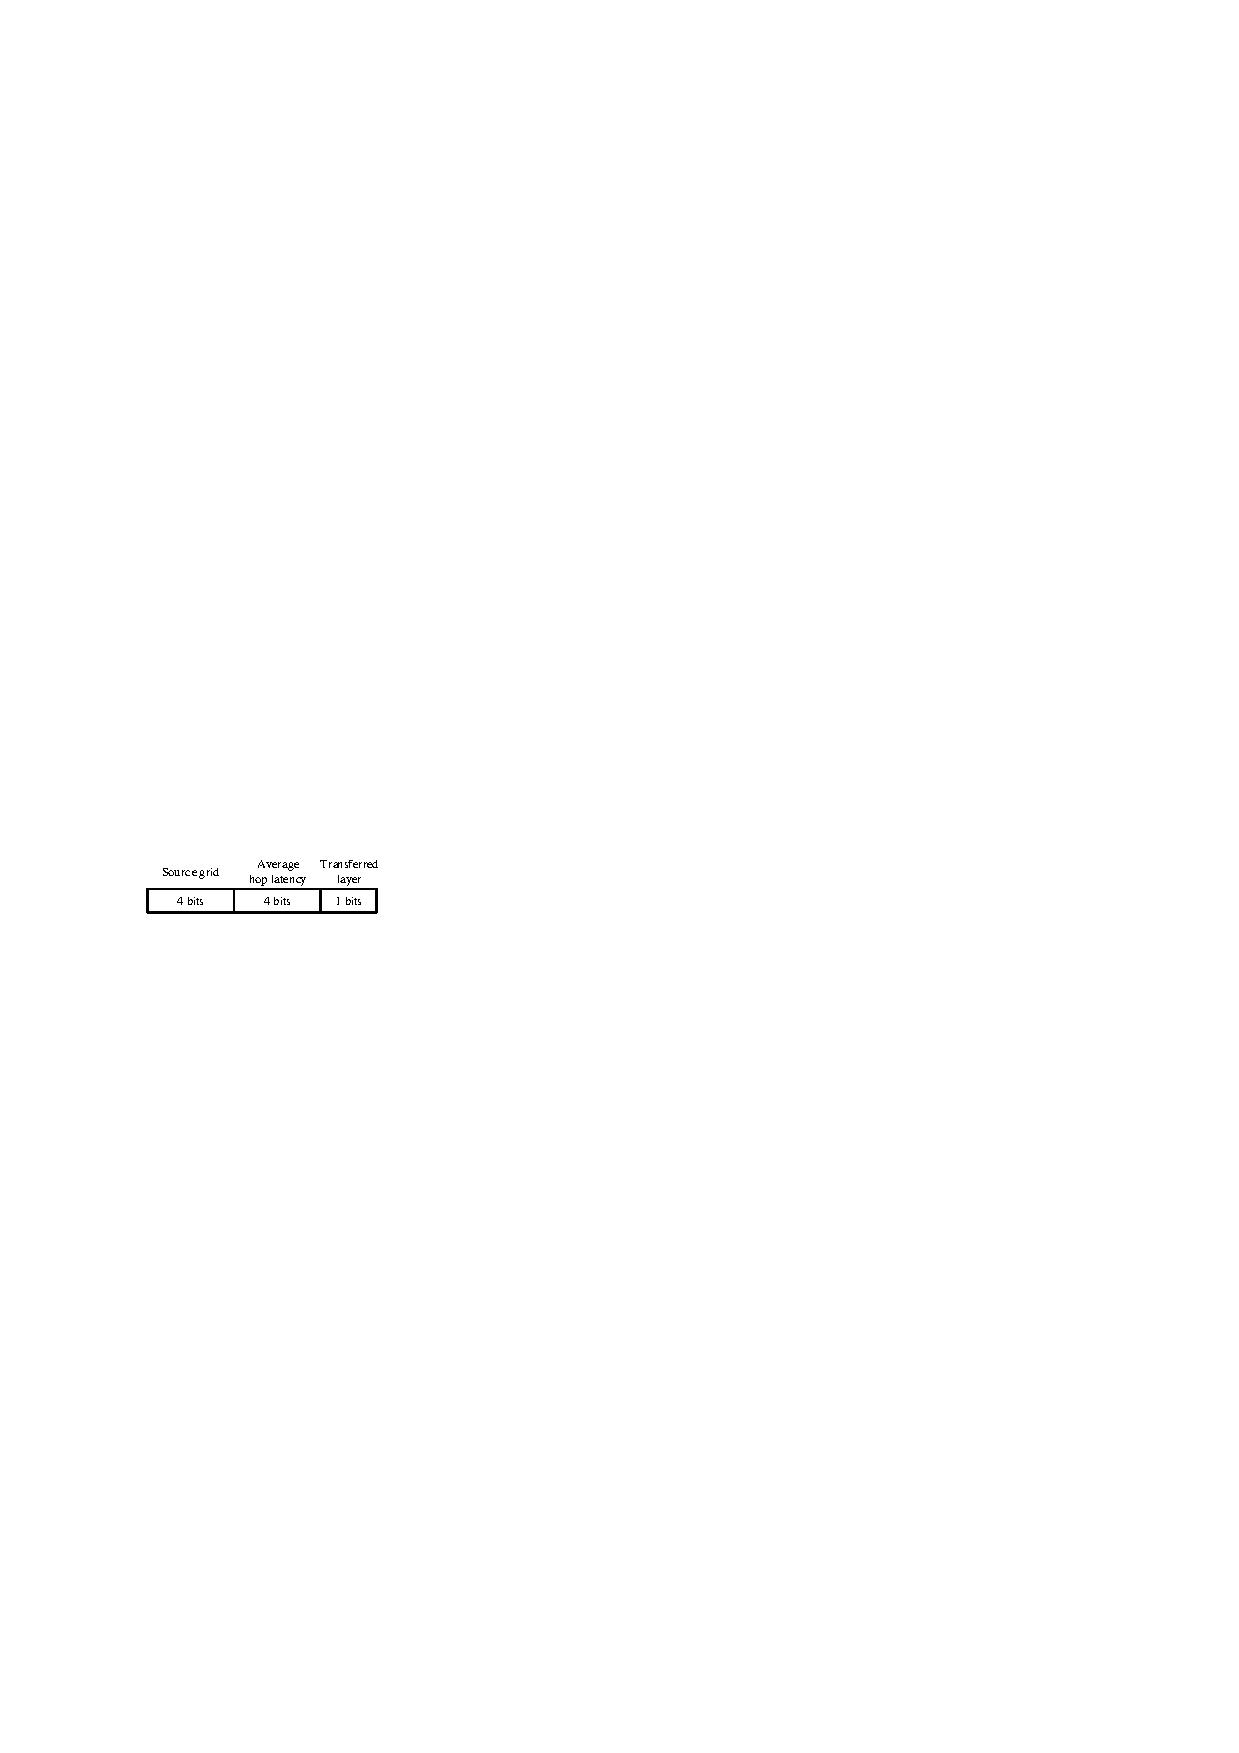
\includegraphics[width=.6\textwidth]{/Figs_DLL/congest_packet}
  \caption{拥塞信息报文}
  \label{fig:congest_packet}
\end{figure}


第三步是传输拥塞信息报文回到源格子。
本章设计了一个完全独立的环网来传输这些报文。
这将在稍后详细介绍。

第四步是计算核比较源格子的每层网络的平均延迟。
根据传输的网络层,源格子将拥塞信息报文存储到两个特定的FIFO中。
这个FIFO有5个空位,采用了最近的5个报文的延迟来计算每个网络层的平均延迟。
根据实验,这五个报文的延迟足够反映出网络的拥塞状态。
由于网络选择是在每个源节点进行的,延迟比较也是在每个源格子进行的。

最后一步是在源节点选择合适的网络层来传输报文。
本章比较了之前步骤计算的每层网络延迟,然后比较结果被发送到该格子的所有节点。
DLL策略动态地发送报文到较轻负载的网络层。
如果CPU层的平均延迟超过硅中介层的平均延迟到一定阈值,硅中介层并不拥塞(硅中介层的平均延迟小于一定阈值),报文发送到CPU层后将被转到硅中介层,继续传输直到报文到达目的节点所在的格子时。
当报文达到目的节点所在格子时,该报文将被发送回CPU层。
在其他情况,每个源节点将发送报文到其默认的网络层。


\subsection{延迟传输环网}
为了能在源节点进行网络层的选择,拥塞信息报文必须从目的节点传输回源节点。
如图~\ref{fig:ring}所示,本章设计了一个延迟传输环网连接着所有的格子以传输这些拥塞信息报文。
这个环网相对独立于当前的网络,因此没有任何相互干扰存在的同时非常高效。
这个独立的环网必须满足两个目标。
第一个目标是\texttt{高带宽}。
一个高带宽的网络允许更多的拥塞信息报文被发送回源格子以获取更精确的拥塞状态信息。
第二个目标则是\texttt{低开销}。
由于环网引入了的是额外开销,因此这些开销必须足够低。
为了满足这两个目标,本章将延迟传输环网设计成多链路无阻塞的形式。
由于环网实现在硅中介层,其面积和连线资源都未被充分利用,环网的开销对于整个系统的影响非常小。

\begin{figure}[htbp] % use float package if you want it here
  \centering
  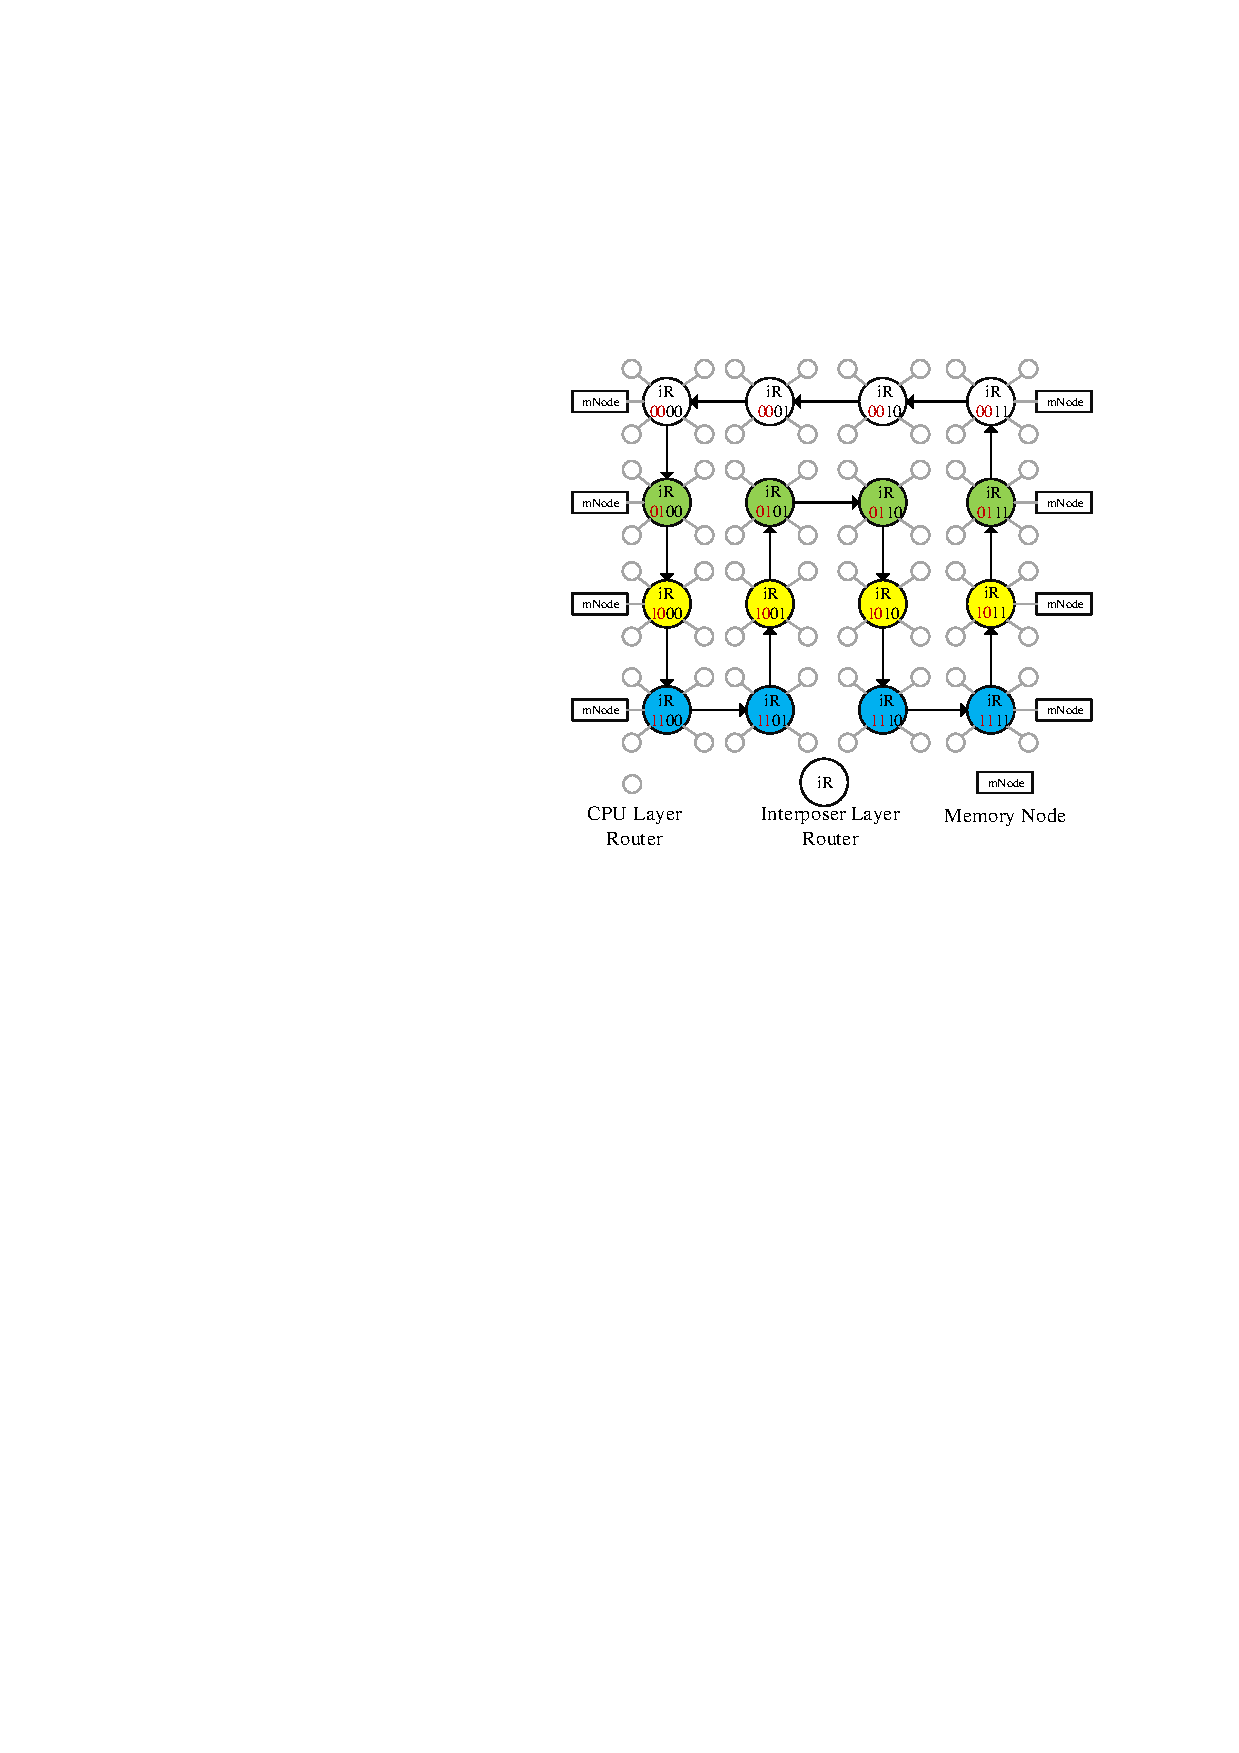
\includegraphics[width=.8\textwidth]{/Figs_DLL/ring}
  \caption{拥塞信息报文传输环网}
  \label{fig:ring}
\end{figure}

\begin{figure}[htbp] % use float package if you want it here
  \centering
  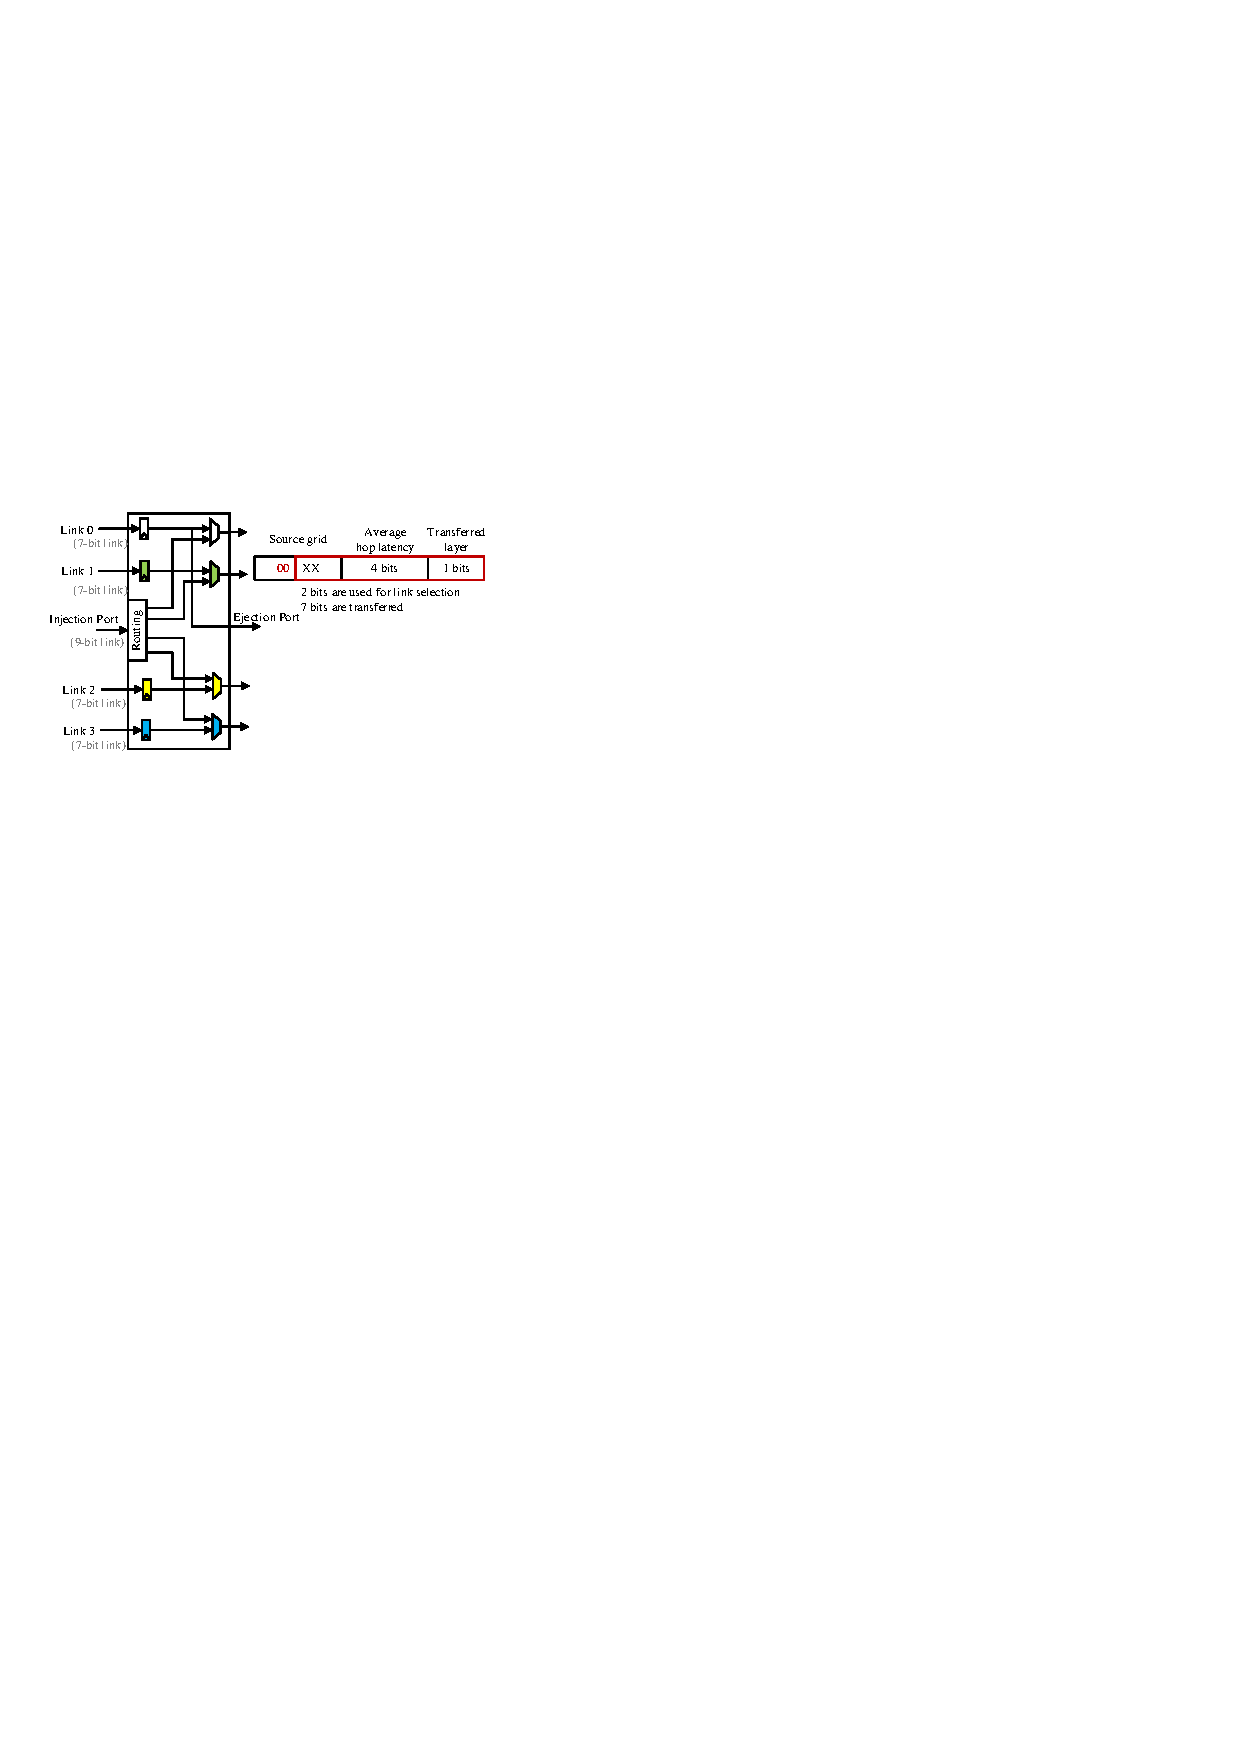
\includegraphics[width=\textwidth]{/Figs_DLL/ring_router}
  \caption{拥塞信息报文传输环网路由器示意图}
  \label{fig:ring_router}
\end{figure}

\textbf{为了获取更高的带宽},本文的延迟环网由四个7位的链路组成。
报文的传输链路由源格子序号(拥塞信息报文的目标格子)的高两位确定。
图~\ref{fig:ring_router}展示了一个格子0的路由器的例子。
如果一个拥塞信息报文被注入格子0,其路由单元会首先选择链路0来传输报文,这是基于源格子ID的高两位\emph{(2‘b00)}确定的。
开始传输后这高两位将被丢弃,只有拥塞信息报文剩下的7位数据需要在环网的链路上传输。
如图~\ref{fig:ring}和图~\ref{fig:ring_router}展示的,被发送到不同颜色格子的拥塞信息报文采用的传输链路也不一样。
通过4条链路,更多的拥塞信息报文可以并行传输。

\textbf{为了降低硬件开销},延迟传输环采用了无缓存路由器结构。
在每个路由器并没有缓存。
在路由器的每条链路上插入一个寄存器,只需要两个时钟周期就能完成一跳步的拥塞信息报文传输。
一旦拥塞信息报文被注入环网,报文将无阻塞地传输到源格子。
为了避免网络层死锁,环网上传输的报文优先级必须高于等待注入的报文的优先级。
换句话说,拥塞信息报文无法在上游路由器有报文的时候注入。

传输拥塞信息报文引入一些延迟。
因为本文提出的延迟传输环网是无阻塞的,这个延迟,拥塞信息能是可接受的够及时的反映当前网络的状态。

在可扩展性方面,目前仅针对64节点的Mesh网络进行设计。
若增加节点规模,需进一步扩展链路规模和拥塞信息报文。
但由于延迟环网的开销非常低,能够满足百核级别的众核互连网络。

\section{实验}
\label{sec:dllexperiment}
采用了时钟精确的互连网络模拟器Booksim~\upcite{jiang2013detailed}进行实验评估。
本章修改了Booksim来实现DLL的2.5维堆叠片上网络结构,通过几种合成流量模型来评估不同的负载均衡策略。
为进一步通过真实应用程序验证实验结果,本文运行了Netrace来评估PARSEC的性能~\upcite{hestness2010netrace}。
本章采用DSENT~\upcite{sun2012dsent}进行面积和功耗模拟。
为了更高效的评估本文提出的DLL策略,本节首先分析了2.5维片上网络结构的瓶颈,因此可以更加深入理解负载均衡策略的性能潜力。
还分析了YX-Z路由策略相比于XY-Z路由策略的优势。
第二,本节比较了DLL策略和没有负载均衡设计的基准设计以及其他两种负载均衡策略。
最后,本节讨论了DLL策略的硬件开销。

\subsection{性能瓶颈分析}

由于2.5维堆叠片上网络结构在CPU层采用了MESH拓扑结构,在硅中介层采用了集中式MESH拓扑结构,而内存节点则在两侧,整个2.5维片上网络结构是不对称的。
因此2.5维堆叠片上网络结构有三个可能的区域会出现瓶颈,包括上层网络、下层网络的中心区域、以及下层网络的边沿区域,如图~\ref{fig:target_system}所示。
任一这些区域都可能导致整个2.5维堆叠片上网络结构的饱和,而实际上很多区域始终在未饱和状态工作。

本文评估了报文传输经过这三块区域的平均延迟。
在基准设计中,采用了XY-Z路由,实验结果如图~\ref{fig:bottleneck}所示。
本文发现上层网络CPU节点在访存报文流量占总流量的25\%会导致全局拥塞。
上层网络的等分带宽是下层网络的两倍。
因此,当访存通信的流量大于总流量的30\%时,下层网络将成为瓶颈。
图~\ref{fig:bottleneck}显示下层网络的边界节点在访存流量大于总流量的30\%时会导致全局网络饱和。
但是,当硅中介层上的边界节点饱和时,硅中介层上的中心节点的报文传输延迟依然非常小,负载也较低。
当访存流量占总流量的75\%时,下层网络的边界部分依然是性能瓶颈。

\begin{figure}[htb]
\centering
\subfloat[访存报文占25\%]{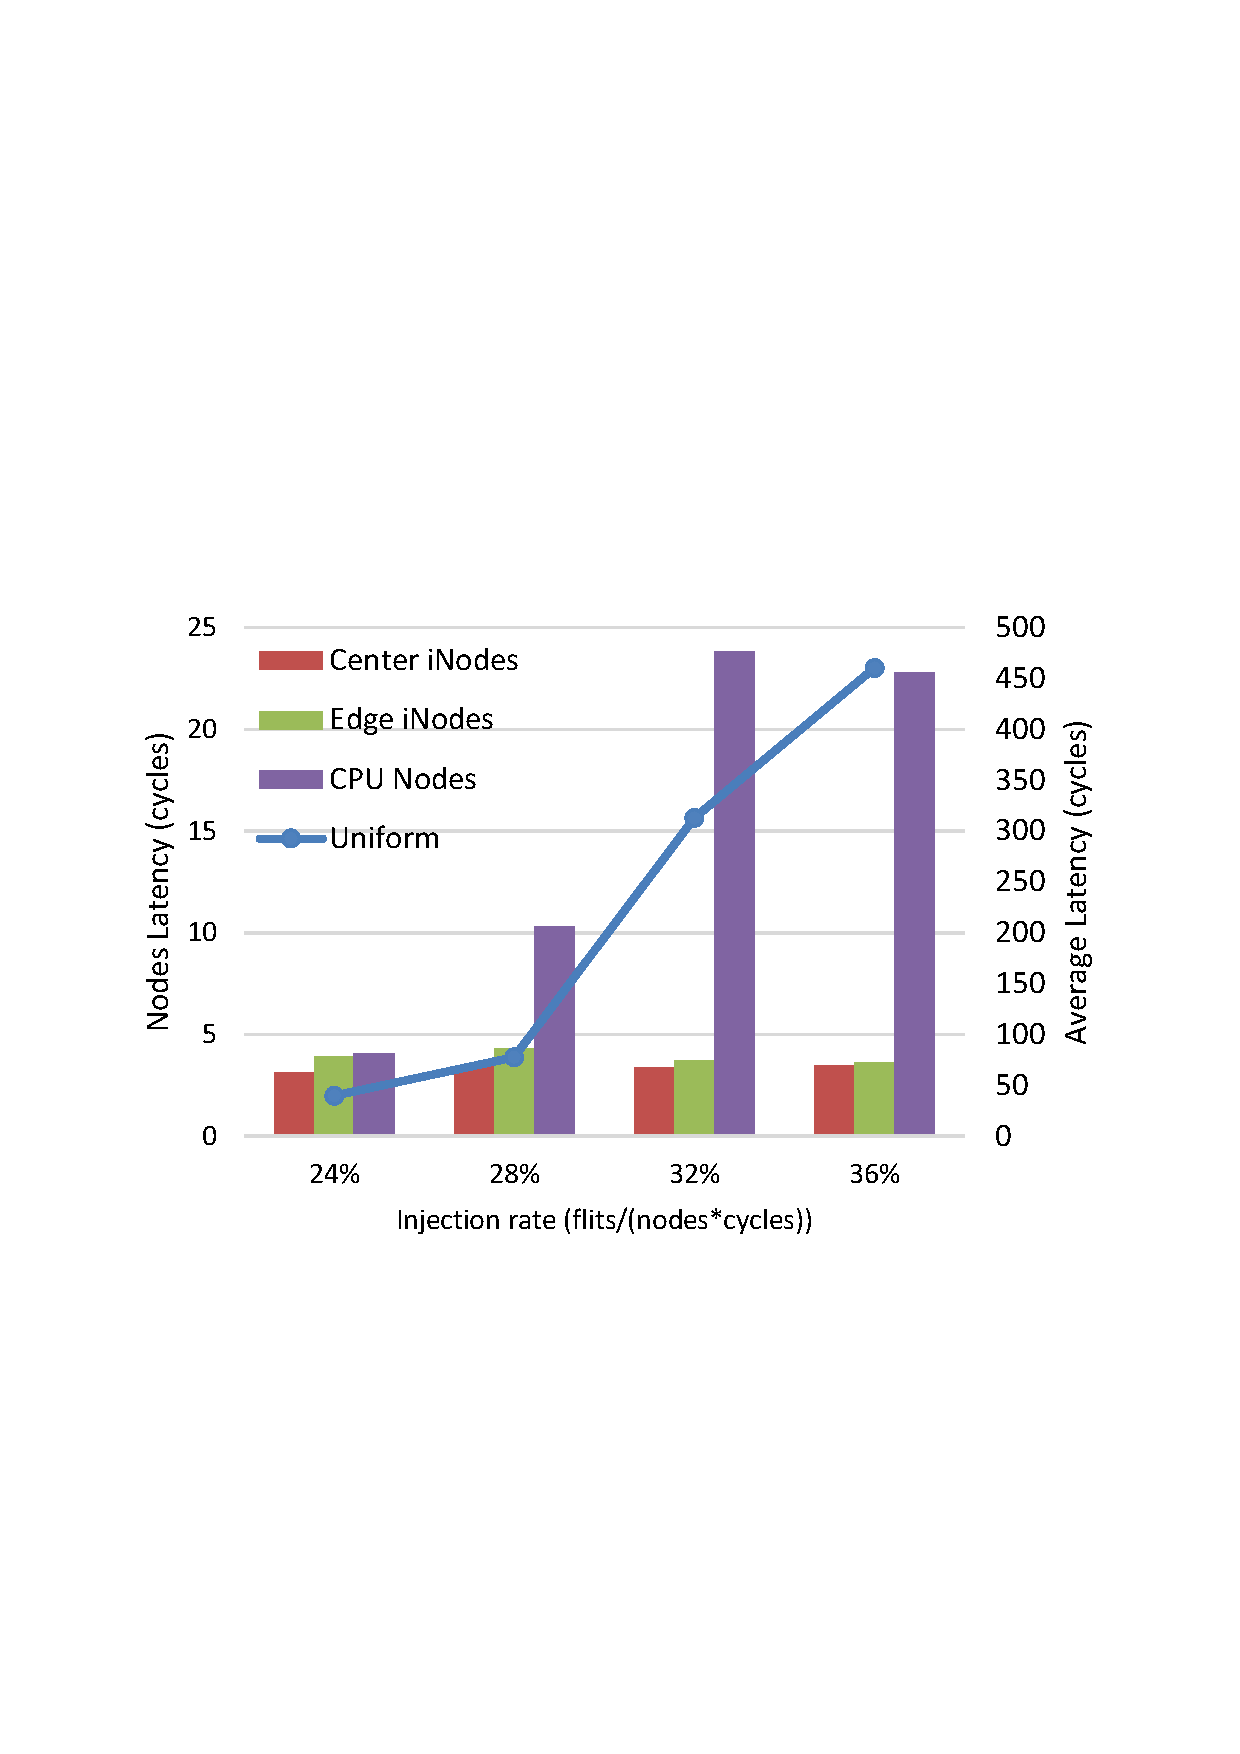
\includegraphics[width=.48\textwidth]{/Figs_DLL/25bottleneck}} 
\subfloat[访存报文占30\%]{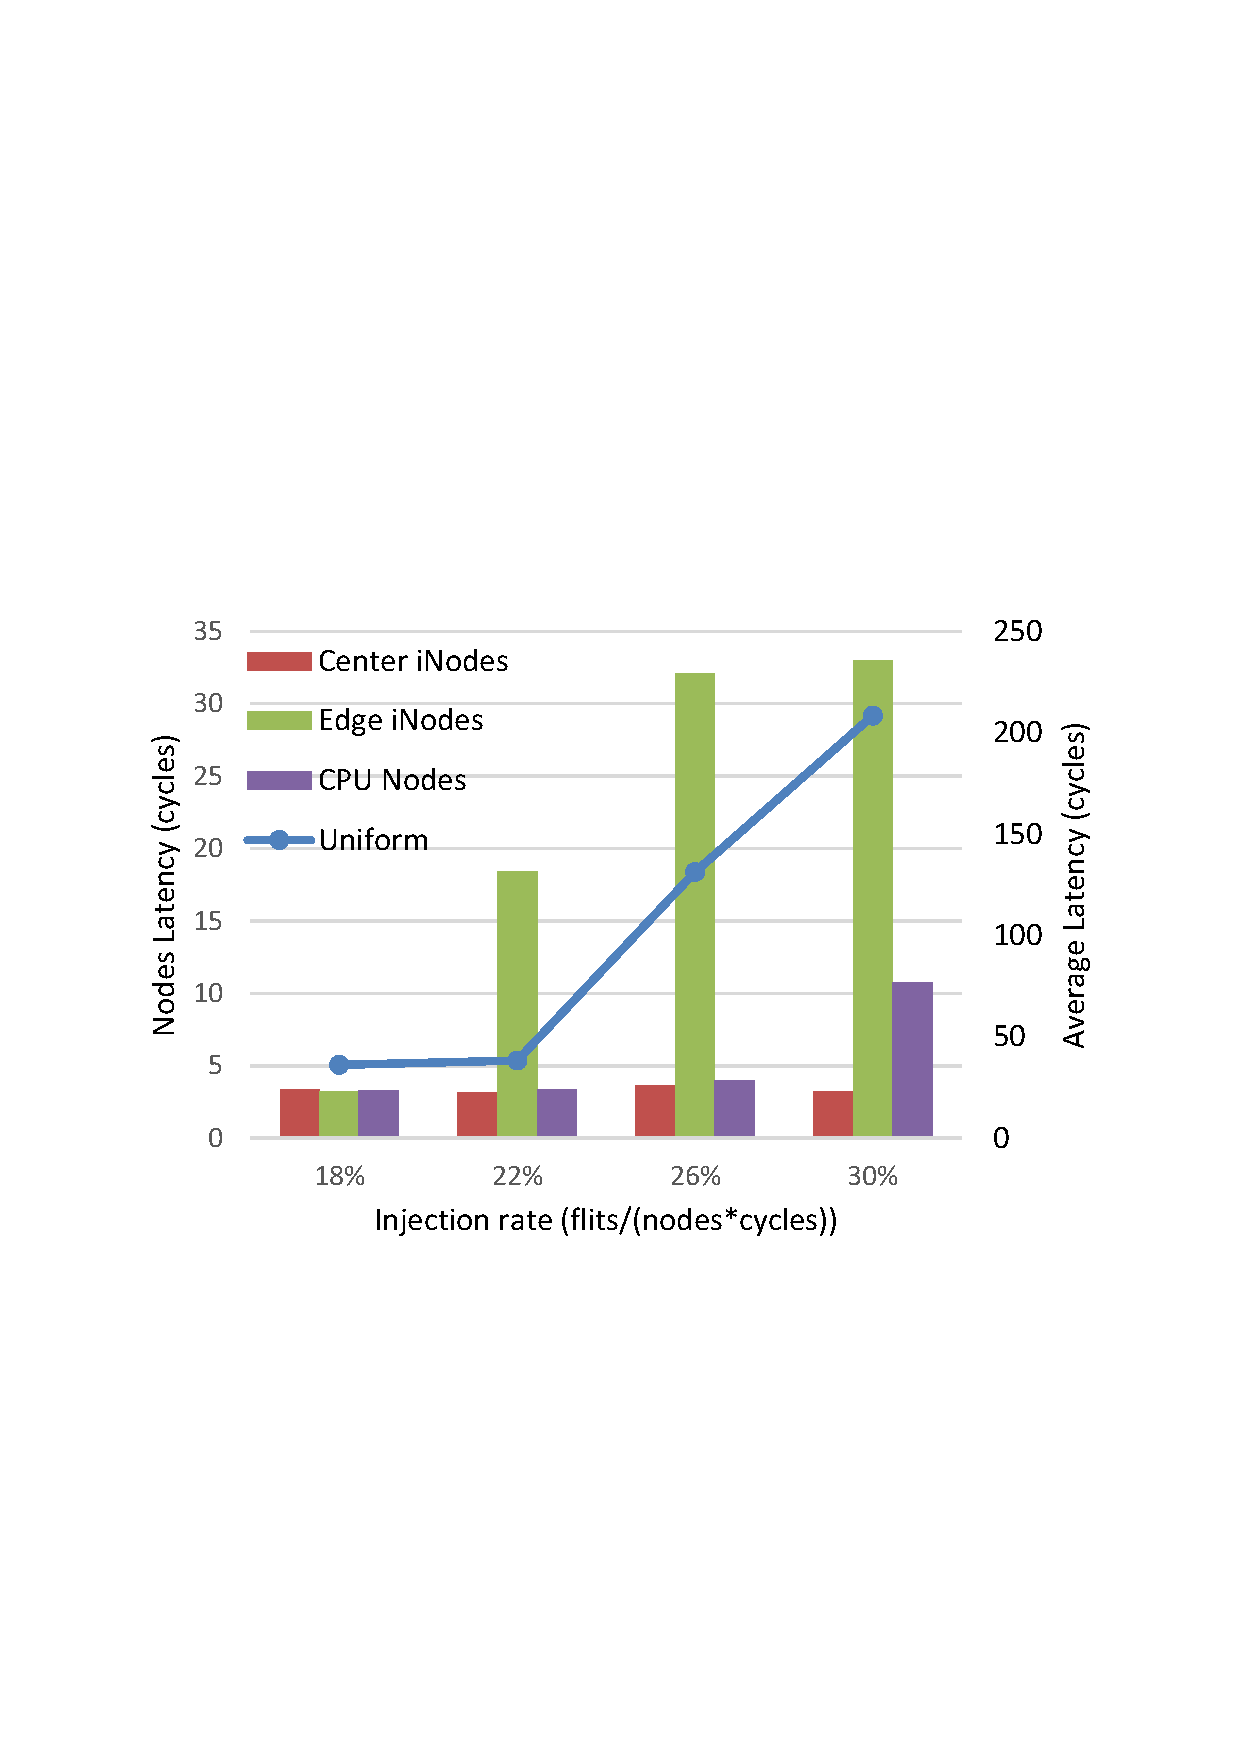
\includegraphics[width=.48\textwidth]{/Figs_DLL/30bottleneck}}\qquad
\subfloat[访存报文占35\%]{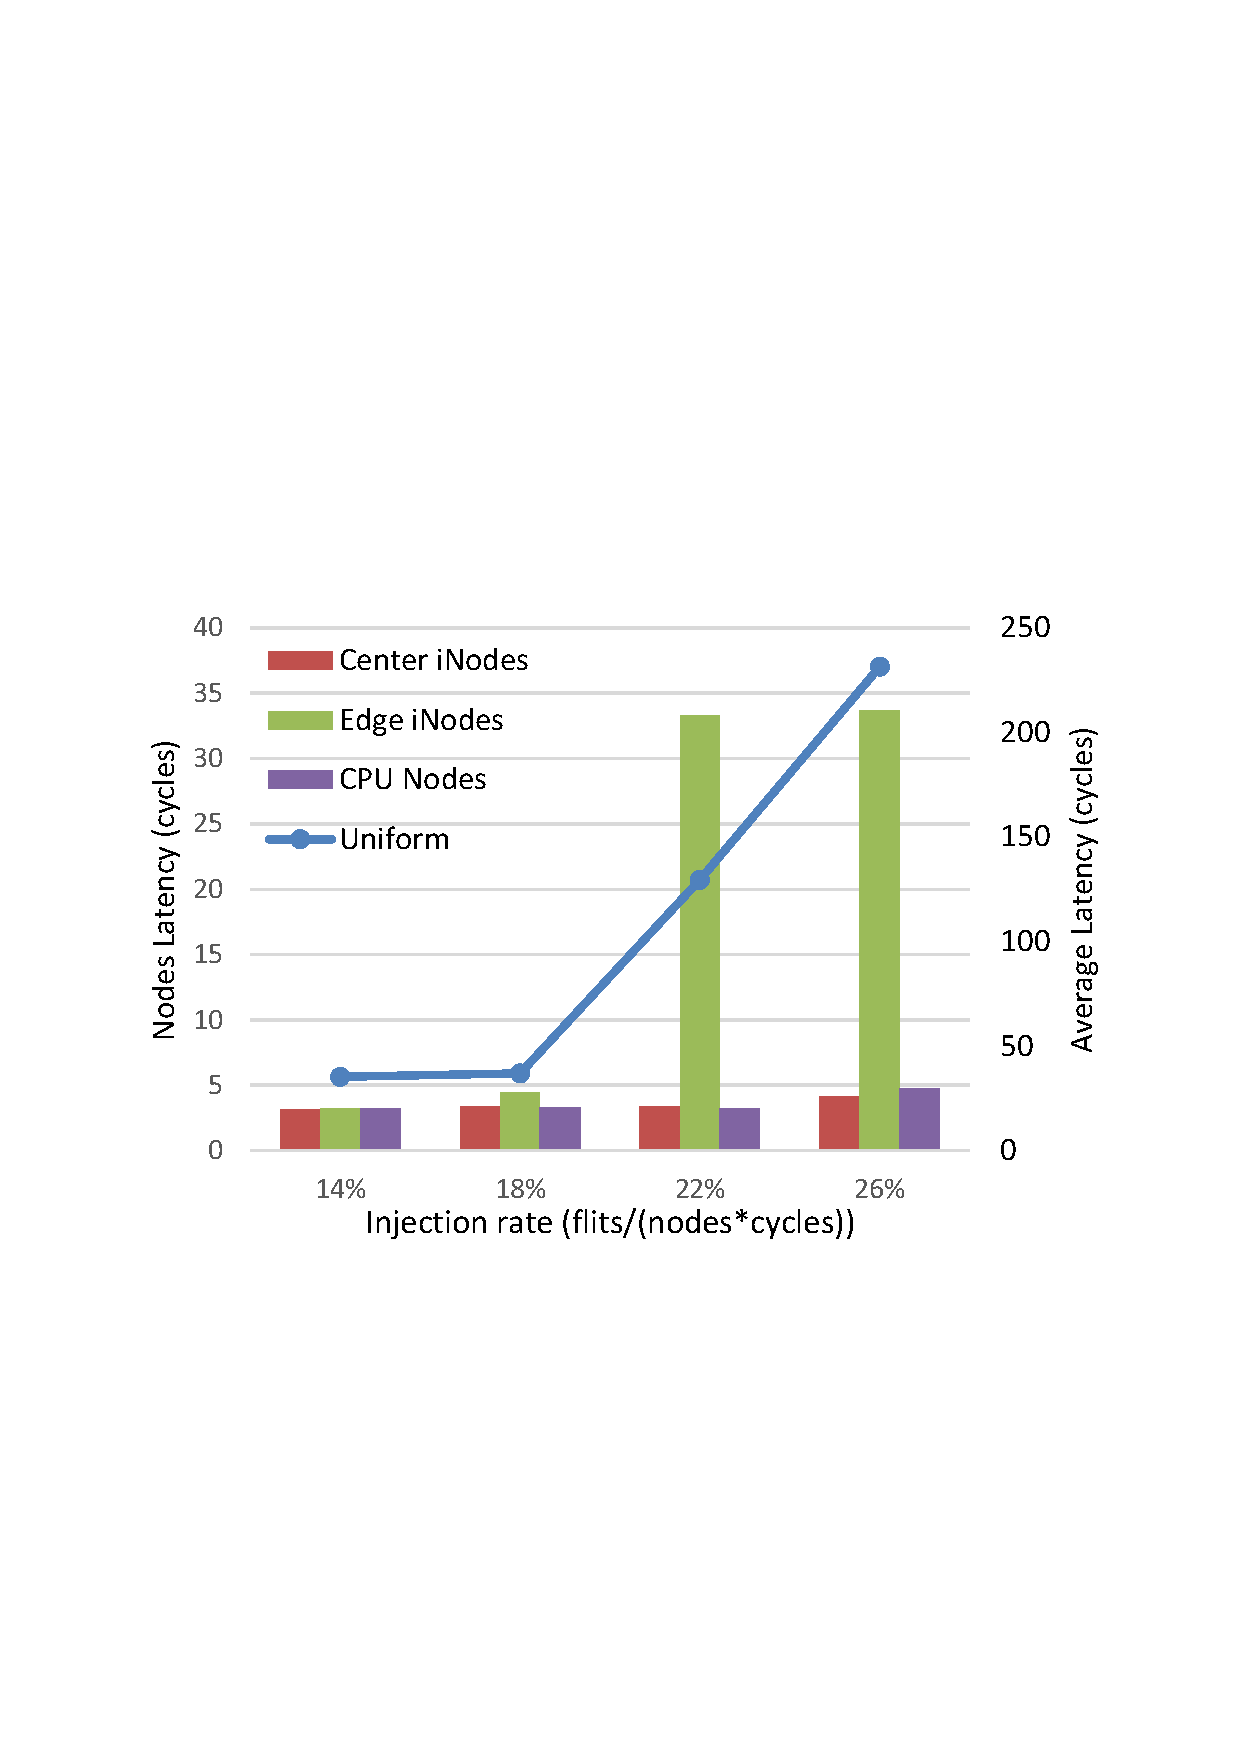
\includegraphics[width=.48\textwidth]{/Figs_DLL/35bottleneck}}
\subfloat[访存报文占75\%]{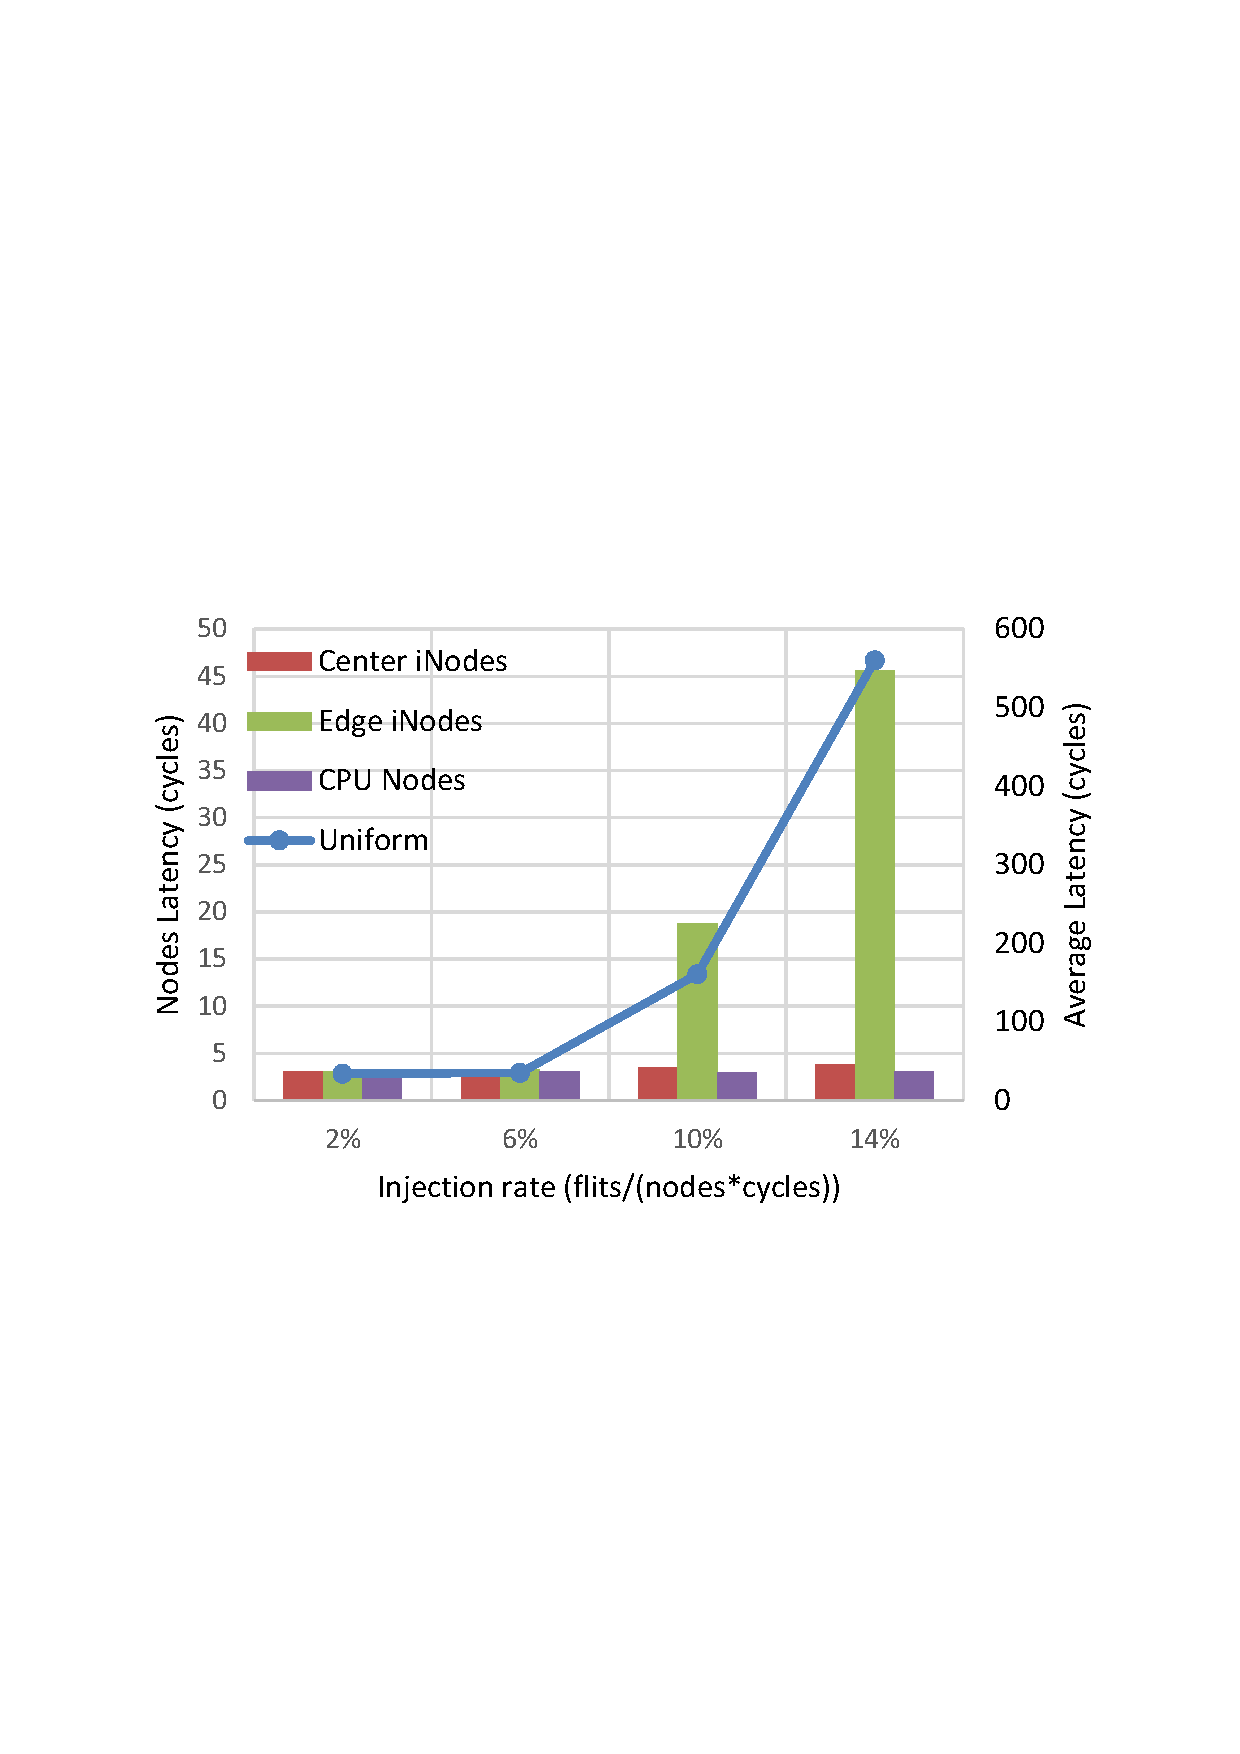
\includegraphics[width=.48\textwidth]{/Figs_DLL/75bottleneck}}  
\caption{性能瓶颈(蓝线表示在Uniform Random通信模型下不同注入率的平均报文延迟;柱形图分别表示不同注入率报文通过不同类型节点的平均延迟。)}
\label{fig:bottleneck}
\end{figure}


幸运的是,这个瓶颈可以通过YX-Z路由来缓解。
YX-Z路由首先将报文沿Y方向传输;这将降低边界列路由器的拥塞。
图~\ref{fig:XYYX}显示当访存流量负载非常重的时候,YX-Z路由相比于XY-Z路由有56.5\%的吞吐率提升。
显然,由于报文先被路由到Y方向,硅中介层网络的两侧边界节点的流量将被显著降低。

\begin{figure}[htbp] % use float package if you want it here
  \centering
  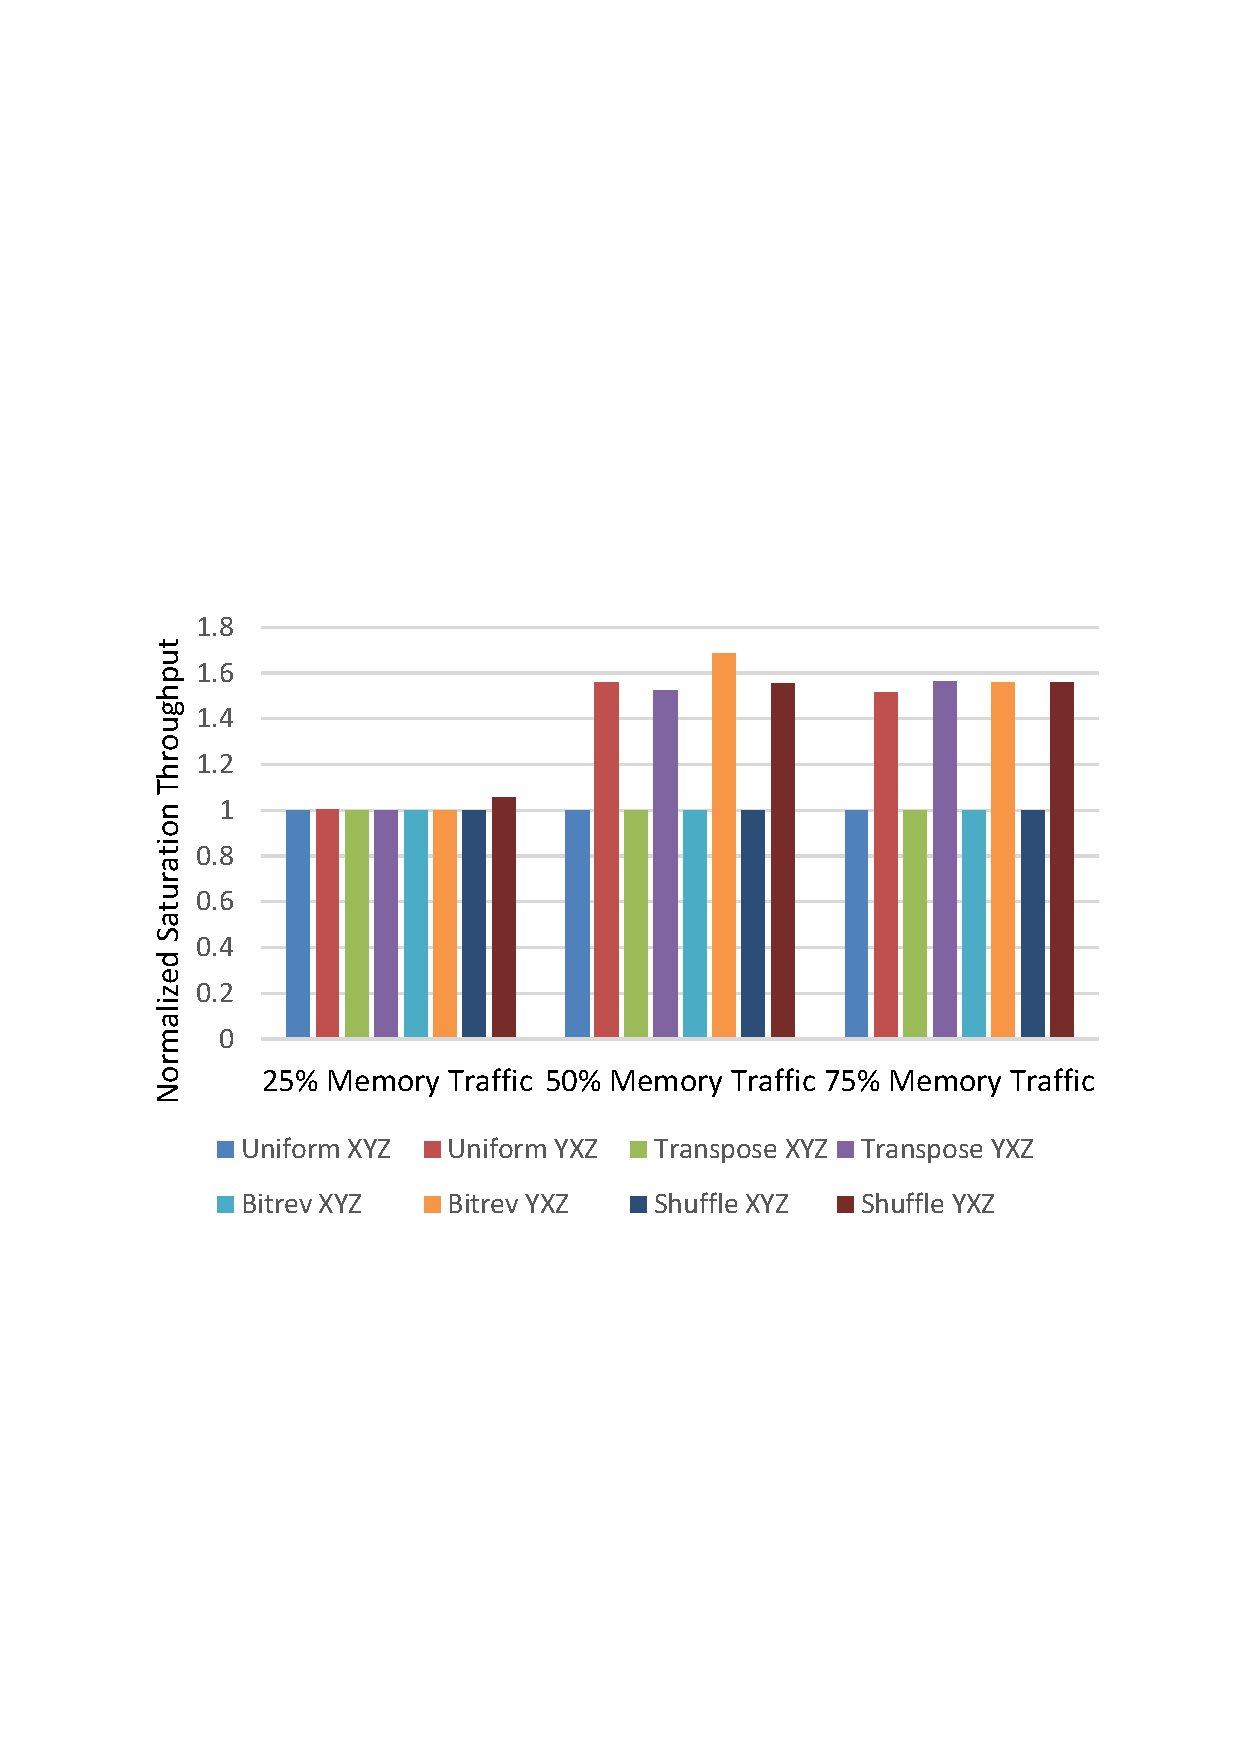
\includegraphics[width=\textwidth]{/Figs_DLL/XYYX}
  \caption{XY-Z路由与YX-Z路由对比(上层网络分别采用四种不同类型的通信模式,下层网络采用Uniform Random的通信模式。)}
  \label{fig:XYYX}
\end{figure}

通过上面的分析,负载均衡策略在访存流量小于总流量的30\%时被应用。
本文评估了PARSEC测试集的应用程序,发现平均访存流量占总流量的14.8\%。
因此,DLL策略对于真实应用程序也会非常有效。

\subsection{性能比较}

在这一小节,本文比较几个不同策略的性能,包括DLL策略、基准设计(DOR)和其他两个负载均衡策略,LoacalBuf和DestDetect。
DOR设计通过不同的网络层传输不同类型的报文。
LocalBuf策略通过路由器缓存占用率来检测本地拥塞。
如果缓存占用率大于60\%,则该路由器被认为是拥塞的。
对于LocalBuf策略,如果上层网络中一个格子内超过一个节点是拥塞的,且硅中介层对应节点不拥塞,核间协议通信的流量将被转入下层以达到负载均衡。
DestDetect策略和DLL策略类似,都是采用延时作为拥塞衡量指标。
该方法收集最近报文的延迟,在目的节点计算每一跳步的平均延迟。
然后目的节点将直接采用收到的报文的平均延迟来指导发送报文的网络层选择。
如果从上层网络收到的报文的延迟大于下层网络收到的报文的延迟到一定阈值,则核间协议通信流量会被转入下层传输。
DestDetect和DLL策略都根据实验选择8个时钟周期作为阈值。
所有的策略都被应用到第~\ref{sec:dlltarget}节描述的目标系统中。
基准路由器采用3级流水线。
为了公平比较的目的,YX-Z路由被应用到所有的策略。

图~\ref{fig:throughput}比较了这些策略在不同访存流量占比的情况下的吞吐率。
结果显示,相比于DOR设计、DestDetect策略和LocalBuf策略,DLL策略分别获得45\%、14.9\%和6.5\%的吞吐率提升。
针对不同的流量模型,DLL策略在Uniform Random流量模型上相比于LocalBuf策略优势很小。
而在Permutation流量模型上,DLL策略的性能则显著好于其他策略。这是因为Permutation的通信模式,流量几乎都是在节点对之间的,这种通信模式对于传输链路的延迟非常敏感。
但是,DestDetect策略的性能相比于LocalBuf策略更差。
这是因为DestDetect策略收集的延迟拥塞信息是收到的报文的路径,而不是报文的发送的路径。
因此,DestDetect策略是一种不准确的方法。
虽然LocalBuf策略不能够反映出拥塞的路径,但本地拥塞信息是准确的。
它比DestDetect的性能更好。


\begin{figure}[htbp] % use float package if you want it here
  \centering
  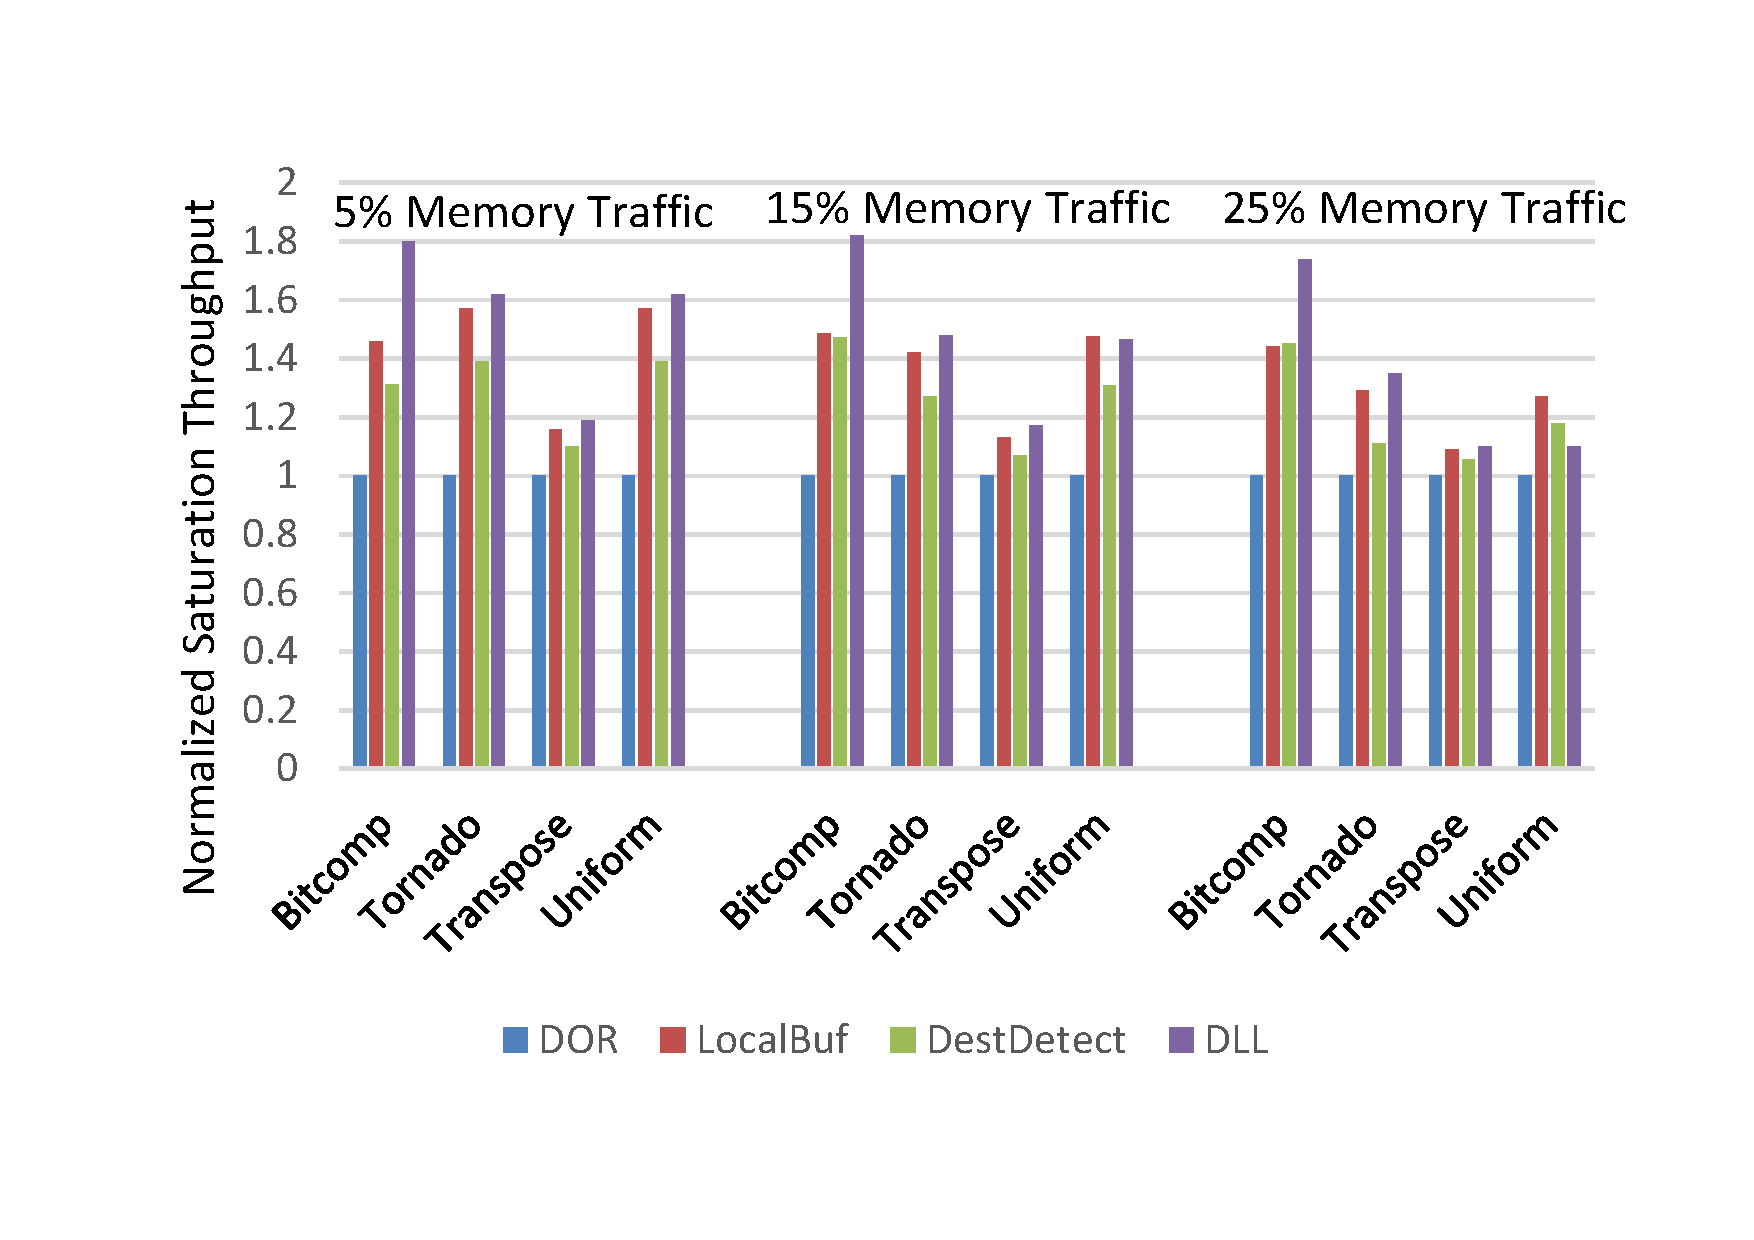
\includegraphics[width=\textwidth]{/Figs_DLL/throughput}
  \caption{吞吐率}
  \label{fig:throughput}
\end{figure}


针对不同的访存通信流量所占百分比。
较小的访存通信流量占比会导致两个网络层更高的不平衡。
两个网络层的流量越不均衡,负载均衡策略就能获得更高的收益。
当访存流量只占总流量的5\%时,DLL策略相比于DOR设计平均有55\%的性能提升。



\begin{figure}[htbp] % use float package if you want it here
  \centering
  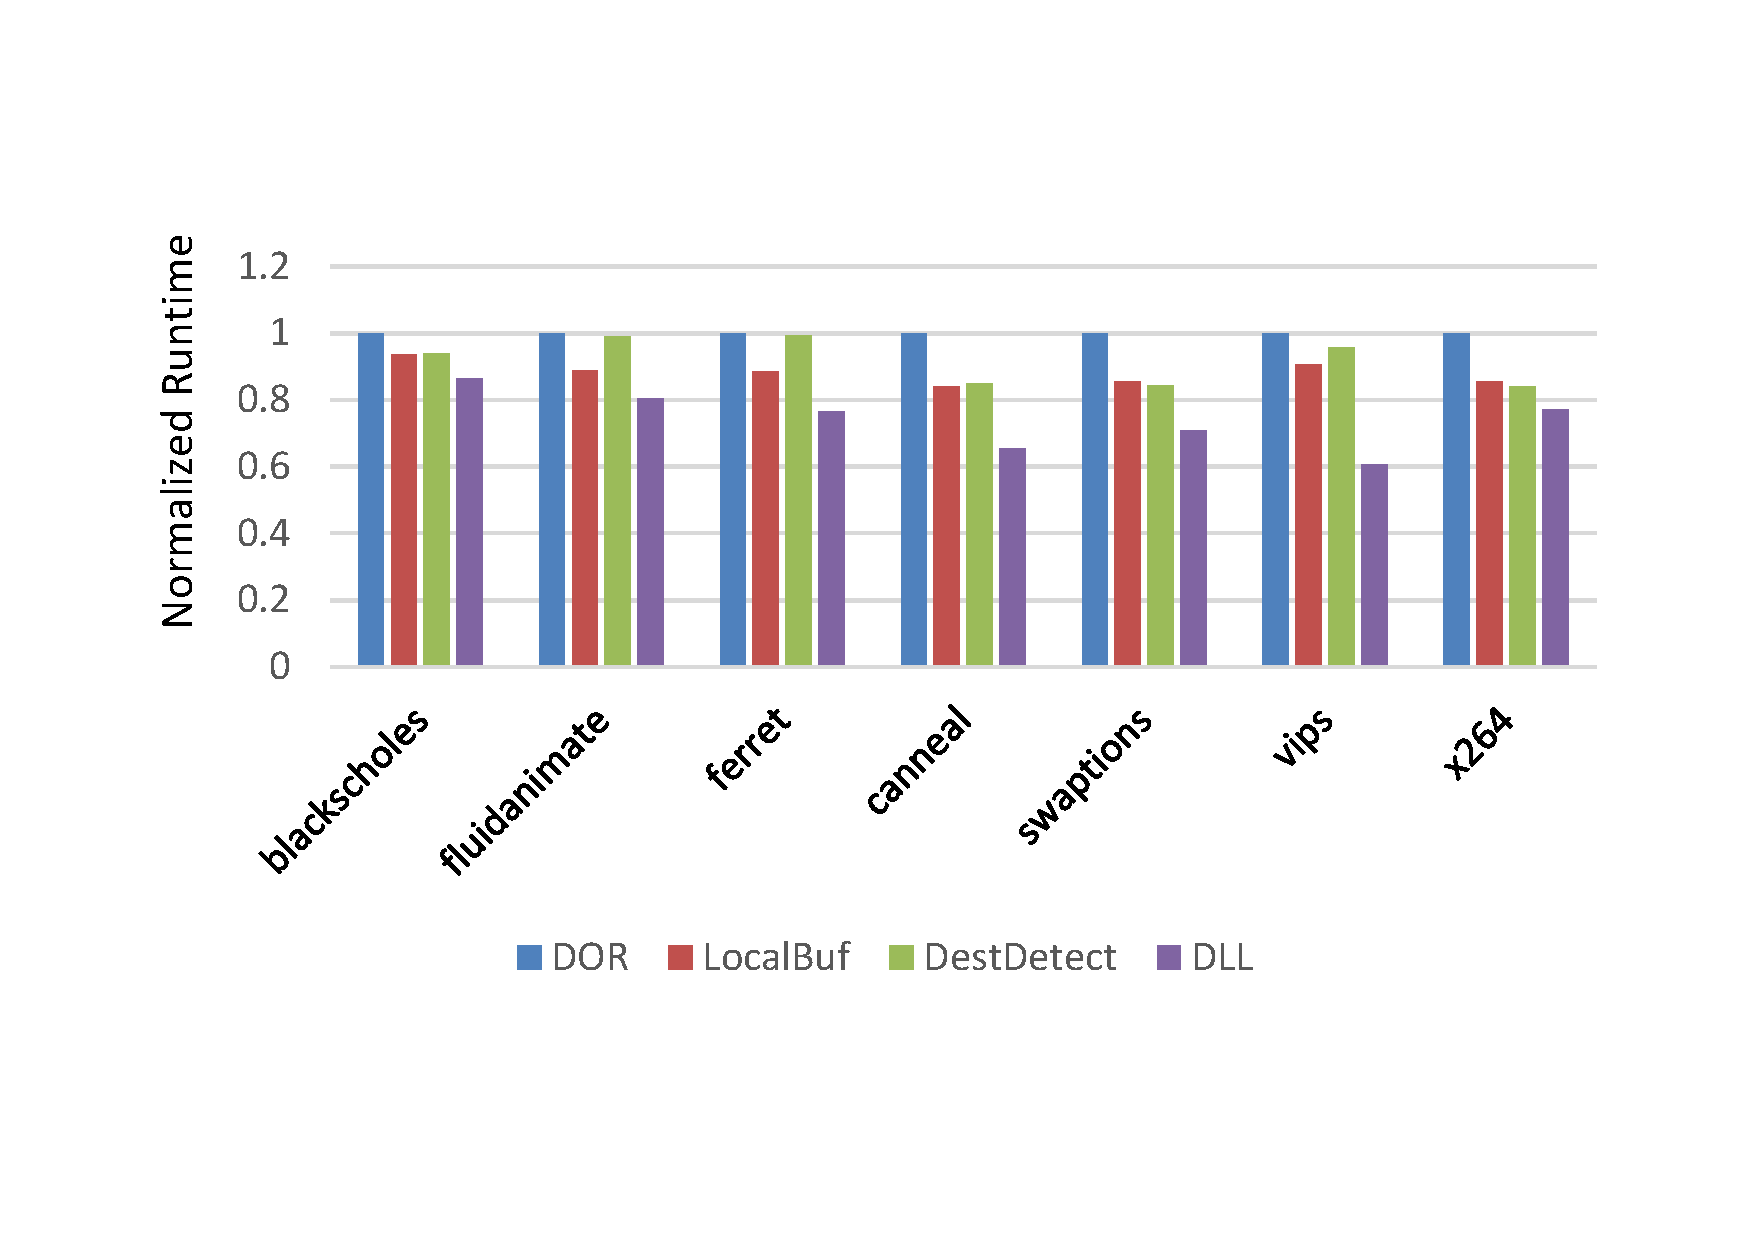
\includegraphics[width=\textwidth]{/Figs_DLL/netrace}
  \caption{Parsec测试集的性能}
  \label{fig:netrace}
\end{figure}

本章还合并了Booksim和Netrace进行真实应用程序的评估。
Netrace中的Trace是从M5模拟器模拟的64核系统中收集的,包括一个64KB的私有一级缓存,一个共享的16MB的二级缓存,以及8个片上存储控制器。
本章评估了PARSEC测试集的所有traces,发现平均访存流量占总流量的14.8\%。
图~\ref{fig:netrace}的结果显示,DLL策略相比于DOR设计平均降低了26.1\%的运行时间,而LocalBuf策略的性能比DestDetect稍高。

\subsection{硬件开销}

图~\ref{fig:hardware}展示了DLL策略相比于DOR设计的硬件开销。
由于LocalBuf策略和DestDetect策略仅仅引入了一点点的逻辑和缓存开销,本章主要评估的是延迟传输环网带来的额外开销。
实验结果是通过在一个45nm bulk/SOI low-Vt 处理节点中采用10\% 切片/节点/时钟周期的注入率收集的。
每个路由器中包含8条虚通道,每条虚通道又包含8个128位的缓存。
图~\ref{fig:hardware}中CPU层的片上网络和硅中介层上的片上网络是逻辑片上网络结构。
硅中介层的实现在短期内都是被动形式。
硅中介层上不存在晶体管。
逻辑上的硅中介层片上网络采用金属线互连,而有源器件(路由器、缓存和中继器)均位于处理器内\upcite{loh2015interconnect}。
这些大量的资源的部署有效提高了性能。
与DOR设计相比,本文的DLL策略多消耗7.7\%的面积和5.8\%的功耗。
事实上,主要的硬件开销来自于延迟传输环网的物理链路和相应存储拥塞信息报文的缓存。
这些缓存和物理链路的开销占用了有源器件的面积和全局连线的面积。
由于本文的延迟传输环网被设计成果无阻塞形式,这些额外的开销很小,是可接受的。

\begin{figure}[htb]
\centering
\subfloat[面积]{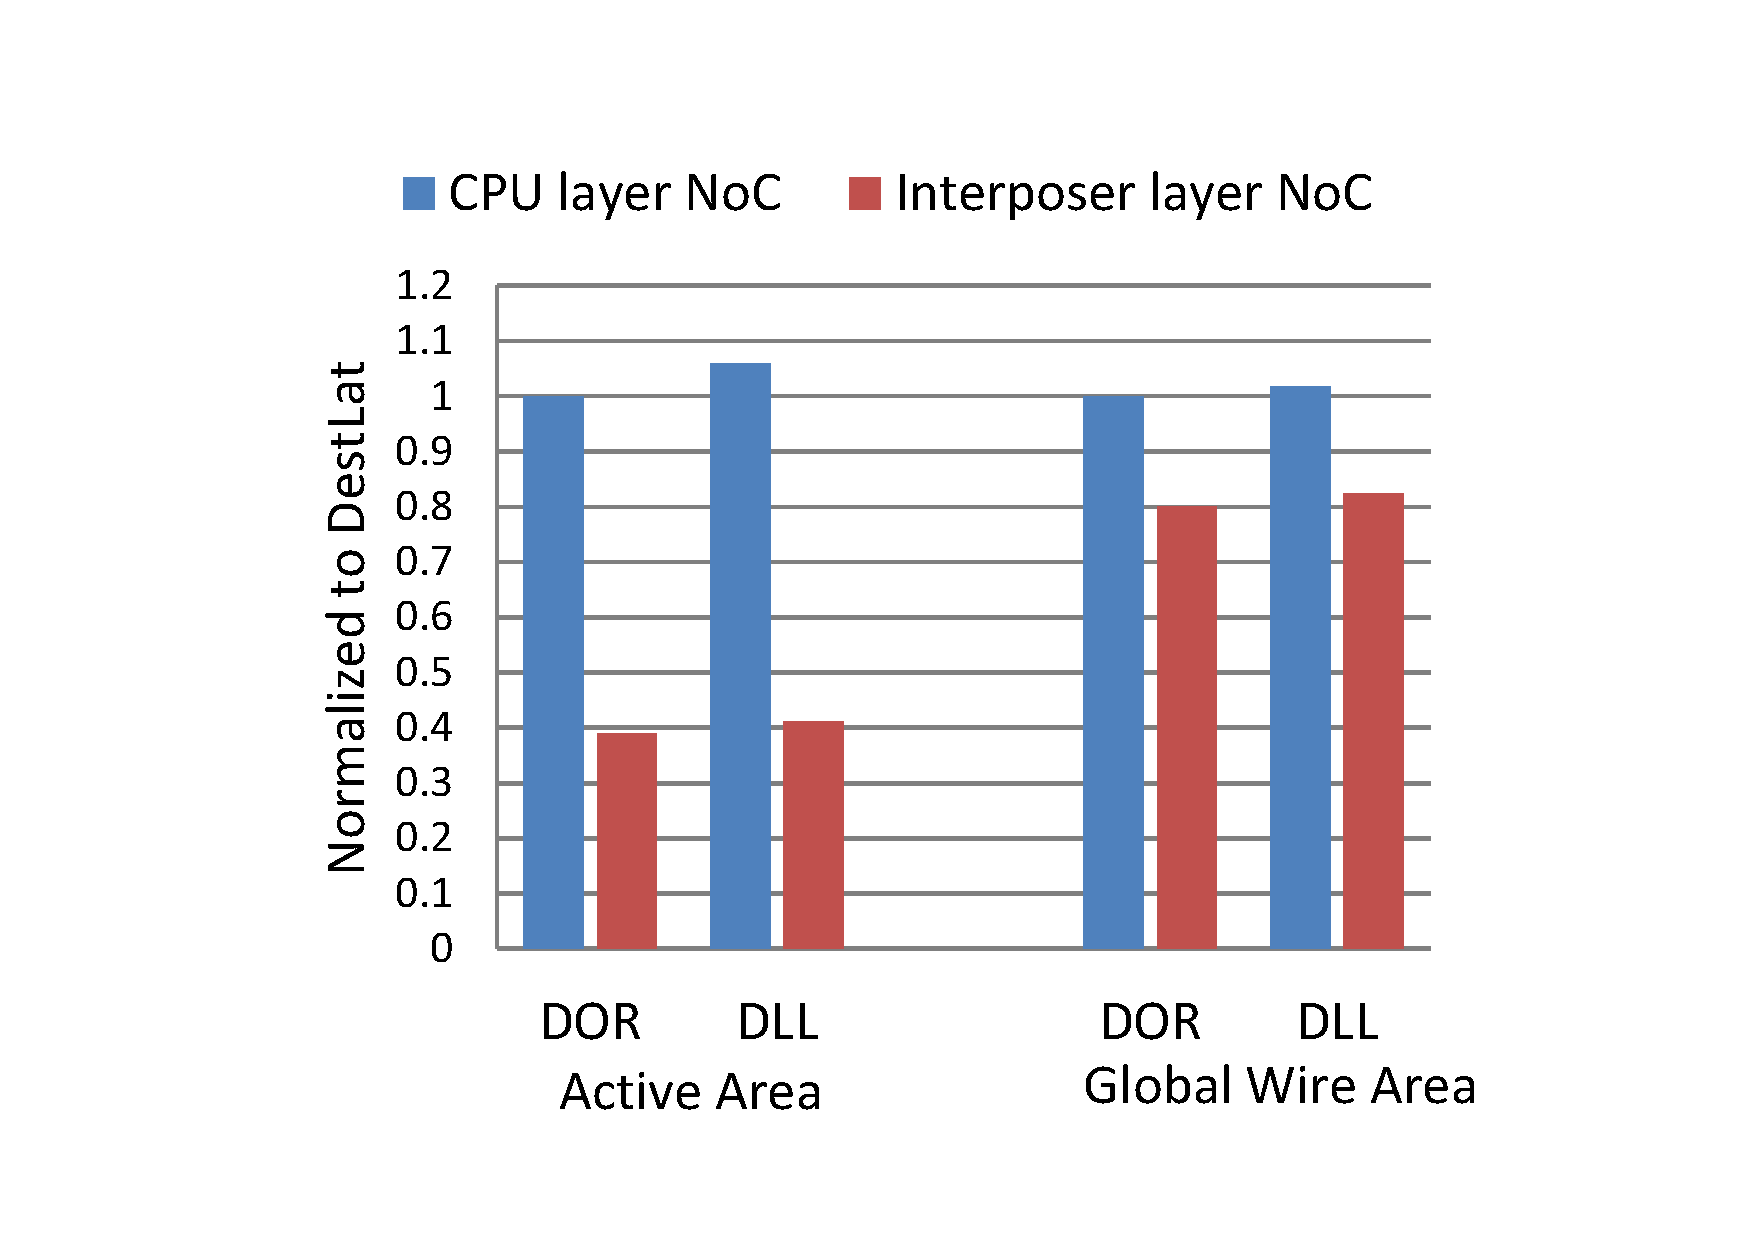
\includegraphics[width=.48\textwidth]{/Figs_DLL/area}} 
\subfloat[功耗]{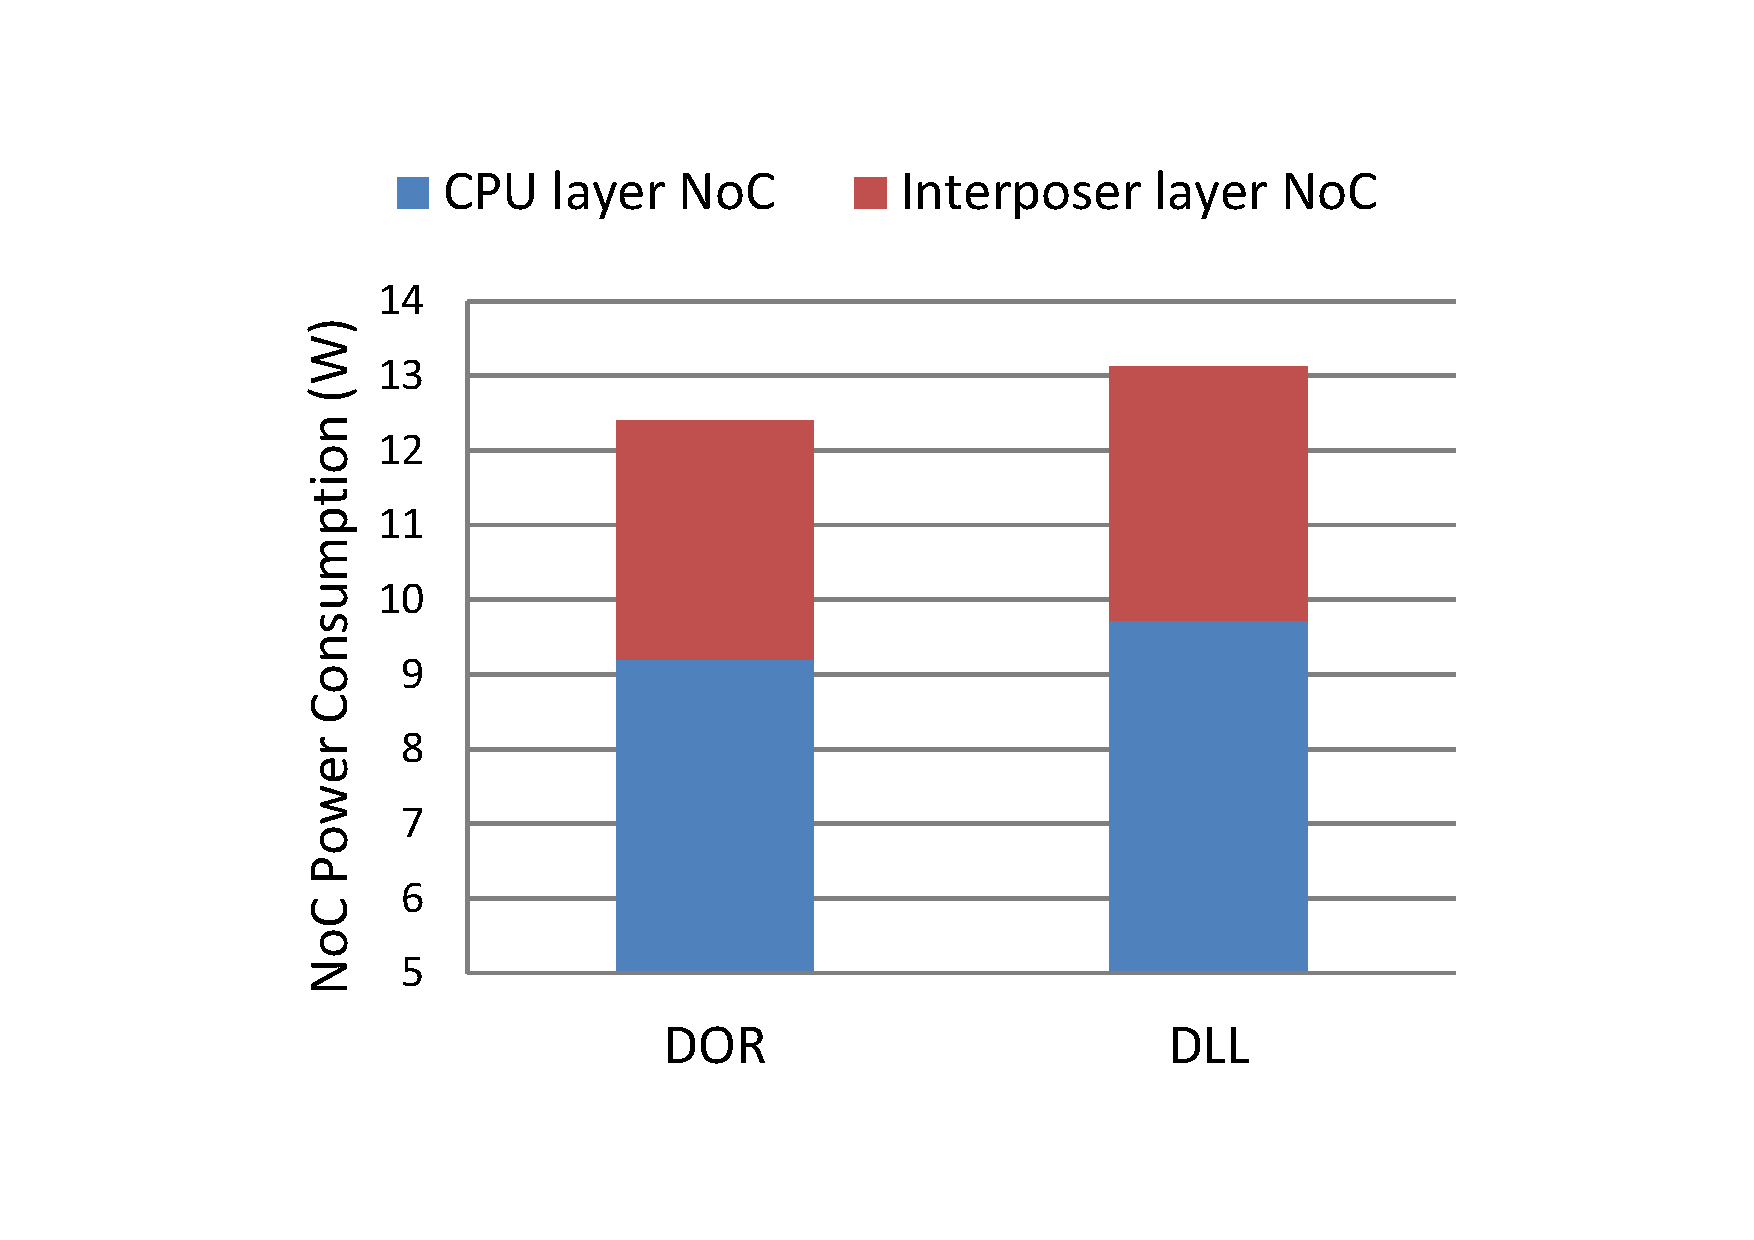
\includegraphics[width=.48\textwidth]{/Figs_DLL/power}}
\caption{硬件开销}
\label{fig:hardware}
\end{figure}


\section{讨论}
\label{sec:dlldiscussion}

在本节,进一步讨论三个细节问题,包括拓扑逻辑,硅中介层的类型和阈值。

首先,2.5维堆叠片上网络可以应用其他的拓扑结构。
Enright Jerger和Kannan等人研究了集中拓扑逻辑~\upcite{jerger2014noc,kannan2015enabling}。
Double-butterflies可以用于解决边界节点的性能瓶颈。
这个拓扑结构减少了冲突并提高了硅中介层网络边界节点的路径多样性。
本章采用了集中式MESH结构显著的降低了$\mu$bump的开销,并且应用了简单的维序路由算法来避免死锁。
这个拓扑结构仅作为负载均衡策略的实现例子。
本文提出的DLL策略可以被应用到其他的拓扑结构,包括Double-butterfly。

第二,硅中介层可以被用来堆叠处理器核存储器。
当前的2.5维堆叠芯片~\upcite{AMD2015USER,black2013stacking}均采用被动式的硅中介层,并不包含有源器件,这种实现仅需要便宜的实现成本和更高的产量。
只有金属连线资源需要被开发,而传输延迟可以在硅中介层网络上被显著降低,这是因为硅中介层采用更宽和更厚的连线。
而长远来看,有源硅中介层的实现可以更好的开发硅中介层上的资源。
本章的目标是提高硅中介层上金属连线的资源利用率。
由于有源器件需要被实现在芯片层,通过应用粗粒度的的方法和无阻塞环网来降低缓存和逻辑的开销。

第三,设置一个合适的阈值是本章的另一个关键点。
本设计的阈值为不同网络层中平均每跳延迟的差值。
如果这个阈值太大,网络对拥塞的反应会很慢。
如果阈值设置的太小,很可能错误的网络选择判断会发生。
但是,不同的流量模型需要不同的阈值。
本章通过一系列实验选择一种适应更多应用程序类型的阈值。
未来,我们会进一步研究反馈策略来动态地调整不同的阈值。



\section{本章小结}
\label{sec:dllconclusion}
2.5维堆叠技术在硅中介层上堆叠芯片和DRAM。
采用硅中介层上的金属线资源,提供了更多的机会去挖掘2. 5维堆叠片上网络结构的新特性。
本章关注到CPU层和硅中介层网络的通信流量不均衡问题,提出了一种动态延迟感知的负载均衡策略DLL。
DLL在每个目的节点收集报文的平均延迟,利用一个多链路无阻塞的环网将延迟信息传输回源节点,为之后的网络选择提供依据以实现负载均衡。
本章评估了不同比例的访存流量来寻找网络瓶颈。
实验结果显示,本章的DLL策略相比于基准设计、DestDetect策略和LocalBuf策略分别有45\%、14.9\%和6.5\%的性能提升。
同时,相比于基准设计,本文的DLL策略仅多消耗7.7\%的面积资源和5.8\%的功耗。
我们之后的工作将会扩展DLL策略以采用适应性阈值设置,并将DLL策略应用到更多的拓扑结构中。